% Options for packages loaded elsewhere
\PassOptionsToPackage{unicode}{hyperref}
\PassOptionsToPackage{hyphens}{url}
\PassOptionsToPackage{dvipsnames,svgnames,x11names}{xcolor}
%
\documentclass[
  super,
  preprint,
  3p]{elsarticle}

\usepackage{amsmath,amssymb}
\usepackage{setspace}
\usepackage{iftex}
\ifPDFTeX
  \usepackage[T1]{fontenc}
  \usepackage[utf8]{inputenc}
  \usepackage{textcomp} % provide euro and other symbols
\else % if luatex or xetex
  \usepackage{unicode-math}
  \defaultfontfeatures{Scale=MatchLowercase}
  \defaultfontfeatures[\rmfamily]{Ligatures=TeX,Scale=1}
\fi
\usepackage{lmodern}
\ifPDFTeX\else  
    % xetex/luatex font selection
  \setmainfont[]{Comic Sans MS}
\fi
% Use upquote if available, for straight quotes in verbatim environments
\IfFileExists{upquote.sty}{\usepackage{upquote}}{}
\IfFileExists{microtype.sty}{% use microtype if available
  \usepackage[]{microtype}
  \UseMicrotypeSet[protrusion]{basicmath} % disable protrusion for tt fonts
}{}
\makeatletter
\@ifundefined{KOMAClassName}{% if non-KOMA class
  \IfFileExists{parskip.sty}{%
    \usepackage{parskip}
  }{% else
    \setlength{\parindent}{0pt}
    \setlength{\parskip}{6pt plus 2pt minus 1pt}}
}{% if KOMA class
  \KOMAoptions{parskip=half}}
\makeatother
\usepackage{xcolor}
\setlength{\emergencystretch}{3em} % prevent overfull lines
\setcounter{secnumdepth}{5}
% Make \paragraph and \subparagraph free-standing
\ifx\paragraph\undefined\else
  \let\oldparagraph\paragraph
  \renewcommand{\paragraph}[1]{\oldparagraph{#1}\mbox{}}
\fi
\ifx\subparagraph\undefined\else
  \let\oldsubparagraph\subparagraph
  \renewcommand{\subparagraph}[1]{\oldsubparagraph{#1}\mbox{}}
\fi


\providecommand{\tightlist}{%
  \setlength{\itemsep}{0pt}\setlength{\parskip}{0pt}}\usepackage{longtable,booktabs,array}
\usepackage{calc} % for calculating minipage widths
% Correct order of tables after \paragraph or \subparagraph
\usepackage{etoolbox}
\makeatletter
\patchcmd\longtable{\par}{\if@noskipsec\mbox{}\fi\par}{}{}
\makeatother
% Allow footnotes in longtable head/foot
\IfFileExists{footnotehyper.sty}{\usepackage{footnotehyper}}{\usepackage{footnote}}
\makesavenoteenv{longtable}
\usepackage{graphicx}
\makeatletter
\def\maxwidth{\ifdim\Gin@nat@width>\linewidth\linewidth\else\Gin@nat@width\fi}
\def\maxheight{\ifdim\Gin@nat@height>\textheight\textheight\else\Gin@nat@height\fi}
\makeatother
% Scale images if necessary, so that they will not overflow the page
% margins by default, and it is still possible to overwrite the defaults
% using explicit options in \includegraphics[width, height, ...]{}
\setkeys{Gin}{width=\maxwidth,height=\maxheight,keepaspectratio}
% Set default figure placement to htbp
\makeatletter
\def\fps@figure{htbp}
\makeatother

\makeatletter
\@ifpackageloaded{caption}{}{\usepackage{caption}}
\AtBeginDocument{%
\ifdefined\contentsname
  \renewcommand*\contentsname{Table of contents}
\else
  \newcommand\contentsname{Table of contents}
\fi
\ifdefined\listfigurename
  \renewcommand*\listfigurename{List of Figures}
\else
  \newcommand\listfigurename{List of Figures}
\fi
\ifdefined\listtablename
  \renewcommand*\listtablename{List of Tables}
\else
  \newcommand\listtablename{List of Tables}
\fi
\ifdefined\figurename
  \renewcommand*\figurename{Figure}
\else
  \newcommand\figurename{Figure}
\fi
\ifdefined\tablename
  \renewcommand*\tablename{Table}
\else
  \newcommand\tablename{Table}
\fi
}
\@ifpackageloaded{float}{}{\usepackage{float}}
\floatstyle{ruled}
\@ifundefined{c@chapter}{\newfloat{codelisting}{h}{lop}}{\newfloat{codelisting}{h}{lop}[chapter]}
\floatname{codelisting}{Listing}
\newcommand*\listoflistings{\listof{codelisting}{List of Listings}}
\makeatother
\makeatletter
\makeatother
\makeatletter
\@ifpackageloaded{caption}{}{\usepackage{caption}}
\@ifpackageloaded{subcaption}{}{\usepackage{subcaption}}
\makeatother
\journal{Elsevier}
\ifLuaTeX
  \usepackage{selnolig}  % disable illegal ligatures
\fi
\usepackage[]{natbib}
\bibliographystyle{elsarticle-num}
\usepackage{bookmark}

\IfFileExists{xurl.sty}{\usepackage{xurl}}{} % add URL line breaks if available
\urlstyle{same} % disable monospaced font for URLs
\hypersetup{
  pdftitle={Building a compendium of expert driven read-across cases to facilitate an analysis of the contribution that different similarity contexts play in read-across performance},
  pdfauthor={Grace Patlewicz; Amanda Ross; HC Bledsoe; Janielle Vidal; Nathaniel Charest; Brett Hagan; Imran Shah},
  pdfkeywords={read-across, regulatory purposes, similarity
context, read-across performance},
  colorlinks=true,
  linkcolor={blue},
  filecolor={Maroon},
  citecolor={Blue},
  urlcolor={Blue},
  pdfcreator={LaTeX via pandoc}}

\setlength{\parindent}{6pt}
\begin{document}

\begin{frontmatter}
\title{Building a compendium of expert driven read-across cases to
facilitate an analysis of the contribution that different similarity
contexts play in read-across performance}
\author[1]{Grace Patlewicz%
\corref{cor1}%
}
 \ead{patlewicz.grace@epa.gov} 
\author[2]{Amanda Ross%
%
}

\author[2]{HC Bledsoe%
%
}

\author[2]{Janielle Vidal%
%
}

\author[1]{Nathaniel Charest%
%
}

\author[1,3]{Brett Hagan%
%
}

\author[1]{Imran Shah%
%
}


\affiliation[1]{organization={Center for Computational Toxicology and
Exposure (CCTE), US Environmental Protection
Agency},city={Durham},country={USA},countrysep={,},postcodesep={}}
\affiliation[2]{organization={ICF
Corporation},city={Reston},postcodesep={}}
\affiliation[3]{organization={Oak Ridge Associated
Universities},city={Oak
Ridge},country={USA},countrysep={,},postcodesep={}}

\cortext[cor1]{Corresponding author}







        
\begin{abstract}
Read-across is a data-gap filling technique utilised to predict the
toxicity of a target chemical using data from similar analogues.
Read-across is predominately performed as part of an expert-driven
assessment which can impede broad acceptance. Data-driven approaches
such as Generalised Read-Across (GenRA) offer scope to generate
reproducible read-across predictions where uncertainties and performance
are quantified. A key issue is how to reconcile an expert driven
approach with a data driven approaches both in terms of how analogues
are identified and evaluated as well as how the read-across prediction
is derived. An important component of analogue identification and
selection is in understanding the contribution that different similarity
contexts play; i.e.~does structural similarity play a larger role in
analogue selection compared with metabolism similarity. This study aimed
to explore some of these considerations through building a compendium of
expert-driven read-across assessments that had been published for
repeated dose toxicity endpoints.
\end{abstract}





\begin{keyword}
    read-across \sep regulatory purposes \sep similarity context \sep 
    read-across performance
\end{keyword}
\end{frontmatter}
    
\setstretch{1.5}
\section{Introduction}\label{introduction}

Read-across is an establised data gap filling technique within analogue
and category approaches that has been used for decades to address
different regulatory purposes. Perhaps the earliest documented example
of read-across was that published by Hanway and Evans in 2000, who
illustrated how to substantiate an analogue approach using acute rodent
oral toxicity and Ames mutagenicity as supporting data. The workflow for
performing read-across has largely remained unchanged over the years
though the introduction of data streams such as high throughput
screening data, transcriptomics, metabolomics data has offered new
possibilities for how source analogues can be identified and evaluated.
The most definitive technical guidance which describes read-across
remains that published by the OECD. Although this was last revised in
2014, a third edition of this guidance will be forthcoming later in 2024
which includes updated sections for how high throughput data can be
used, how uncertainty can be characterised and documented as well as
updates for specific types of analogue/category approaches including
nanomaterials, UVCBs and metal containing substances. One limitation
with the technical guidance notwithstanding this anticipated update is a
lack of case studies to demonstrate what a successful and robust
read-across assessment should resemble. The guidance has certainly
benefited from the examples under the OECD IATA Case studies project but
up until now there has not been a concerted effort to collect examples
to showcase what robust read-across looks like, what level of supporting
information is warranted and how this might differ depending on the
decision context and/or the regulatory jurisdiction.

The EU's REACH guidance offers additional indirect guidance for how ECHA
assesses read-across cases based on its own read-across assessment
framework (RAAF) but there are no published examples indicating which
dossiers were successful. Read-across practioners have only the RAAF for
indirect guidance and access to the published ECHA decision letters that
document shortcomings in dossiers. Identifying which dossiers have
utilised read-across is not a trivial undertaking. Tracing back the
dossier and cross referencing the associated decision letters tend to
describe shortcomings in the dossier beyond read-across, e.g.~poor
substance characterisation. In Patlewicz et al (2024), an algorithmic
approach was undertaken to help identify dossiers where read-across had
been performed at least for oral repeated dose study outcomes but the
study fell short of identifying how many of the dossiers had been
ultimately successful in the application of read-across. Moreover even
having identified the dossiers and the specific source analogue used in
each case, the rationale behind the identification, evaluation and
justification of those analogues remained opaque. The study record
relying on a source substance was known such that an association between
that and the target substance could be established but an assumption had
to be made as far as whether those source substances arose from a
category or analogue approach could not be readily made, moreover the
process by which candidate analogues were identified and rationalised to
make a determination that the source substance data was sufficient to
address the data gap was not available. That said, the study did shine a
light on some of the challenges with current read-across in terms of a
disconnect between a regulation stipulating that structurally similar
analogues should be identified yet finding that many of the source
analogues ultimately used were often not particularly structurally
similar or that in the majority of cases, a more similar analogue could
have been selected. Most likely reasons for this disconnect are due to
the absence of access to available toxicity data. Nonetheless the study
was a useful exploration of the ways in which analogues could be
characterised and compared relative to their target substances. Assuming
the read-across inference itself was sufficient for purpose - in many
cases using a structure-based algorithmic approach gave rise to similar
predictions of toxicity.

In this study, a concerted effort was made to do a targeted literature
search of primary and grey literature to identify read-across cases
where the approach had been accepted either for the stated context of
interest or at least where there had been more documentation to justify
the entire workflow from the strategy of the candidate analogues, by
which tools or expertise and how those were subsequently evaluated for
the endpoint of interest. The study was limited to repeated dose
toxicity outcomes and focused on the oral route of exposure to mitigate
variability in the types of read-across scenarios under consideration.
The aims of this study are several fold: 1) firstly conduct a targeted
literature search to gather as many read-across examples as possible. 2)
define a schema to capture relevant information in a harmonised and
machine readable format and lastly 3) investigate different ML
approaches to evaluate the similarities of the analogues identified as
well as ways in which these could be codified for predictive profiling.

\section{Materials and Methods}\label{materials-and-methods}

\subsection{Identification of read-across
examples}\label{identification-of-read-across-examples}

Initially read-across cases were compiled from the EPA Provisional Peer
Review Toxicity Values (PPTRV) assessments (https://www.epa.gov/pprtv),
OECD IATA case studies
(https://www.oecd.org/chemicalsafety/risk-assessment/iata/) and OECD
High Production Volume (HPV) categories
(https://hpvchemicals.oecd.org/UI/Search.aspx). A web query was created
in python to query each of the \textasciitilde400 PPRTVs (first accessed
June 2021) and identify only those PPRTV assessments where an Appendix A
was available in the final report as this was a crude proxy for whether
a read-across assessment might have been performed. Each of the 37 cases
initially identified were then manually checked and information
extracted from the reports themselves. The HPV examples were reviewed to
identify only those cases where there was a SIAR assessment for only
categories containing members that were discrete organic substances.
Inorganics were considered out of scope. All OECD IATA case studies
tagged as read-across were identified and each was extracted where the
endpoints of interest were repeated dose toxicity outcomes.

A preliminary literature search was conducted based on selected authors
who were well known to have published on read-across such as Nicholas
Ball, Karen Blackburn, Sharon Stuard, Terry Schultz, Mark Cronin, Grace
Patlewicz and Sylvia Escher amongst others. A more comprehensive
literature search was subsequently conducted against Pubmed using the
Abstract Sifter Tool version 7 using the following search query term
\texttt{"Read-across\ {[}tiab{]}\ OR\ Read\ across\ {[}tuab{]}\ OR\ Chemical\ grouping\ {[}tiab{]}\ OR\ Category\ Approach\ {[}tiab{]}\ or\ category-approach\ {[}tiab{]}\ OR\ Analogue\ approach\ {[}tiab{]}\ OR\ Analog\ approach\ {[}tiab{]}\ OR\ Surrogate\ approach\ OR\ Grouping\ concept{]}"}.
This netted 934 results as of 18th July 2023. Each of the abstracts were
then manually reviewed and tagged yes/no or maybe. Certain articles were
potentially duplicative of cases already extracted based on selected
authors or already captured as part of the IATA Case studies or HPV
categories. These were tagged as far as possible. Approximately 100
articles were labelled as Yes with a further 76 as maybes for subsequent
extraction. The full articles were then sourced and screened to
determine whether they met minimal criteria of including a read-across
assessment for a repeated oral toxicity endpoint.

\subsection{Schema to capture the
Information}\label{schema-to-capture-the-information}

A structured excel sheet was created to capture relevant information
from each case. This included the target substance(s) being assessed,
the candidate source analogues, the toxicity value information being
read across, as well as the rationale used to identify and evaluate the
analogues (so-named analogue evidence streams). A Standard Operating
Protocol (SOP) was drafted to document the approach in an effort to
ensure consistency in the extractions. Extractions were performed by one
individual which were then checked for completeness and consistency by a
second individual. The SOP was updated as necessary to capture revisions
as the bread of case studies changed. This was inevitable given the
HPVs, PPRTVs and IATA Case studies were structured per specific
templates whereas there was more variability in terms of how literature
studies described any read-across.

\subsection{Chemical information}\label{chemical-information}

Since many of the evaluations to be explored were chemical specific, the
read-across cases information needed to be augmented with structural
information for both target and source analogues. Target and source
analogue identities were queried using the EPA CompTox Chemicals
Dashboard to retrieve CASRN identifiers and structures using SMILES as
well as DSSTox Substance Identifier (DTXSID) information.

\subsection{Landscape Evaluation}\label{landscape-evaluation}

A initial summary overview of the read-across cases was performed to
better understand the landscape of the chemicals under study, the use
cases explored, whether a category or analogue approach had been
employed, and what tools or approaches were used to identify analogues.
The freely available web application ClassyFire was used to categorise
all discrete organic structures into classes using its own chemistry
ontology.

\subsection{Similarity context
evaluation}\label{similarity-context-evaluation}

Similarity contexts evaluated included structure, structural alerts,
physicochemical properties and predicted metabolism. Similarity in
structure relied upon generation of Morgan chemical fingerprints using
the open source python library RDKit, constructing a pairwise distance
matrix using Jaccard as the metric. Structural alerts were generated
using the Derek Nexus version 2.5 by batch processing all substances
using default settings. The union of all unique endpoint-toxicophore
combinations was first extracted and a dataframe constructed with all
substances as rows and all endpoint-toxicophore combinations as columns.
If a substance presented an alert combination, the dataframe cells were
populated by a 1 to denote presence of an alert and otherwise 0 to
denote absence of an alert. Physicochemical properties relied upon using
OPERA predictions of LogKow, calculated MW, number of Hydrogen Bond
donors and Acceptors. A pairwise distance matrix using a normalised
Euclidean distance was then calculated. The metabolism of the substances
were simulated using the OASIS TIMES \emph{in vitro} rat liver model.
Using the tree report output based on default settings, metabolic
similarity was then quantified in three ways: 1) evaluating the
similarity in actual metabolites produced by each substance, 2)
evaluating the pairwise similarity using the transformation pathways
produced for each substance and 3) evaluating the similarity of the
actual simulated metabolic graph using the graph kernel similarity
metric, WL.

\subsection{Quantifying the contribution of similarity
contexts}\label{quantifying-the-contribution-of-similarity-contexts}

A Bayesian logistic regression was created to investigate the
contribution of the different similarity contexts and quantifying the
distributions of their coefficients. Substances that were members of a
read-across case were tagged as similar whereas substances between cases
were tagged as dissimilar. This created a highly imbalanced dataset with
only 2665 combinations of pairs as similar and 101,937 as dissimilar. To
balance the dataset so that the number of pairs were evenly split, the
dissimilar pairs were downsampled randomly so that a equal number of
similar and dissimilar pairs set remained. This balanced set was then
split 75:25 into a training: test set. The training set was subjected to
a Bayesian logistic regression whereas the test set was reserved to
evaluate overall performance in the predictions. The logistic regression
was set up such that the target outcome (whether a pair of substances
were similar) was assumed to follow a Bernouilli distribution with logit
as the logistic function. To build the Bayesian logistic regression,
normally distributed priors were set for each for the different
similarity metrics (Structural similarity, Alert similarity,
Physicochemical similarity, WL similarity, metabolites similarity and
transformation similarity). Once priors were specified, posterior
distributions were used to approximate the posterior distributions using
Markov Chain Monte Carlo simulations. The PyMC library in python was
used to draw samples from the posterior. The sampling algorithms used
was NUTS, in which parameters are tuned automatically.

\subsection{Bayesian Networks}\label{bayesian-networks}

Approaches to explore BBN for the analogue approaches? For consideration

\subsection{Metric learning
approaches}\label{metric-learning-approaches}

\subsubsection{Deep learning approaches}\label{deep-learning-approaches}

A deep learning metric learning approach was attempted as follows: A
pairwise matrix was constructed for all substances with SMILES. If a
pair of substances were both members of the same read-across case, it
was denoted by label 0, otherwise a label 1 was assigned. Since the
number of dissimilar pairs was so much greater than the number of
similar pairs, a random sampling was performed to downsample the number
of dissimilar pairs to create a balanced dataset. A Graph Isomorphism
Network (GIN) within the pytorch geometric library was then constructed
using a Siamese network architecture such that a pair of substances
could be fed into the network, the contrastive loss could be used as the
loss function to learn the embeddings in which two similar substances
had a low Euclidean distance and two dissimilar points had a large
Euclidean distance. Target-analogue SMILES were used as inputs which
were converted into pytorch-geometric graphs to extract embeddings
representing both chemical structure information that could be
predictive of whether an analogue pairs was part of the same read-across
case or not. A Graph Convolutional Network was also constructed using a
Siamese network architecture but in this case, 2 pytorch objects
constructed based on the predicted metabolic graph using the same TIMES
\emph{in vitro} model where the nodes were the parent/metabolites and
the edges the transformation pathway.

\subsubsection{Shallow learning
approaches}\label{shallow-learning-approaches}

An Informational Theoretic Metric Learning (ITML) approach was also
attempted using a paired learning approach. This relied on using a pair
of similar or dissimlar substances with the aim of deriving an embedding
that would discriminate dissimilar from similar pairs using Malanhobis
as the distance metric. ITML minimises the (differential) relative
entropy, aka Kullback-Leibler divergence, between two multivariate
Gaussians subject to constraints on the associated Mahalanobis distance,
which can be formulated into a Bregman optimization problem by
minimizing the LogDet divergence subject to linear constraints. The
balanced dataset was split randomly into a test set and training set
using a 80\%:20\% ratio. A 5-fold CV approach was undertaken to assess
mean CV performance. A grid search was then undertaken to identify the
best hyperparameters whilst generalising the performance. In the ITML
approach, Morgan chemical fingerprint representations were used to
characterise the analogue pairs.

\subsubsection{UMAP}\label{umap}

A different way of representing the input data was to take the
difference between the analogue pairs and fit a UMAP to learn an
embedding that would separate substance pairings that were similar from
those that were dissimilar using Morgan chemical fingerprints as an
input. A supervised UMAP approach was undertaken using 5 neighbours and
a Jaccard metric. The supervised embedding was then applied into a
Support Vector Machine as classifier fit analogue pairs. A 10 fold cross
validation strategy was used to evaluate the performance using balanced
accuracy as a test metric. The model was refitted to the training set
and applied to the 25\% test set that had been left out during training
and testing.

\section{Results and Discussion}\label{results-and-discussion}

\subsection{Schema for the Dataaset}\label{schema-for-the-dataaset}

to be done

\subsection{Dataset Summary}\label{dataset-summary}

Currently, 82 read-across assessments were extracted from three main
sources. There were 22 unique decision contexts which were then grouped
by 3 main types - New Approach Methods (NAMs), technical guidance or
regulatory purposes. For the 82 examples, 68 cases (82\%) were developed
to meet a regulatory purpose, the remainder were relatively evenly split
between efforts to improve existing technical guidance (10\%) or
illustrate the utility of NAMs to substantiate read-across
justifications (7\%). The balance of decision contexts is not
unsurprising given the origin of the case studies, \textasciitilde25
(30\%) of the cases were taken from the US EPA PPRTV effort, 38\% were
OECD SIDs examples, 15\% were OECD IATA case studies, 10\% from journal
articles with the remainder comprising a couple of examples each from
ECETOC or Health Canada. Of the approaches used, there was a bias
towards category approaches with 55\% of cases utilising a category
approach and 36\% being analogue approaches. All the EPA PPRTV cases
relied on an analogue approach whereas in general over 90\% of all other
examples used a category approach.

\subsection{Chemical Landscape}\label{chemical-landscape}

In terms of the chemical landscape, the read-across cases captured 498
unique substances of which structures could be mapped for 467 of them.
For the substances without structures, these were all UVCBs arising from
11 different studies drawing from the OECD IATA and SID examples. For
the 467 substances with SMILES, the ClassyFire service was used to tag
each substance with a superclass, class annotation to summarise the
types of functional classes captured by the read-across cases.
ClassyFire superclasses Benzenes and substituted derivatives (25\%),
Fatty Acyls (14\%), Carboxylic acids and derivatives (12\%) as well as
Organooxygen compounds (12\%) captured \textasciitilde63\% of all the
chemicals. A t-SNE plot \textbf{?@fig-tsne} based on Morgan chemical
fingerprints colour coded by the most populist chemical superclasses
illustrates the read-across landscape to provide some perspective of the
makeup of the chemistry.

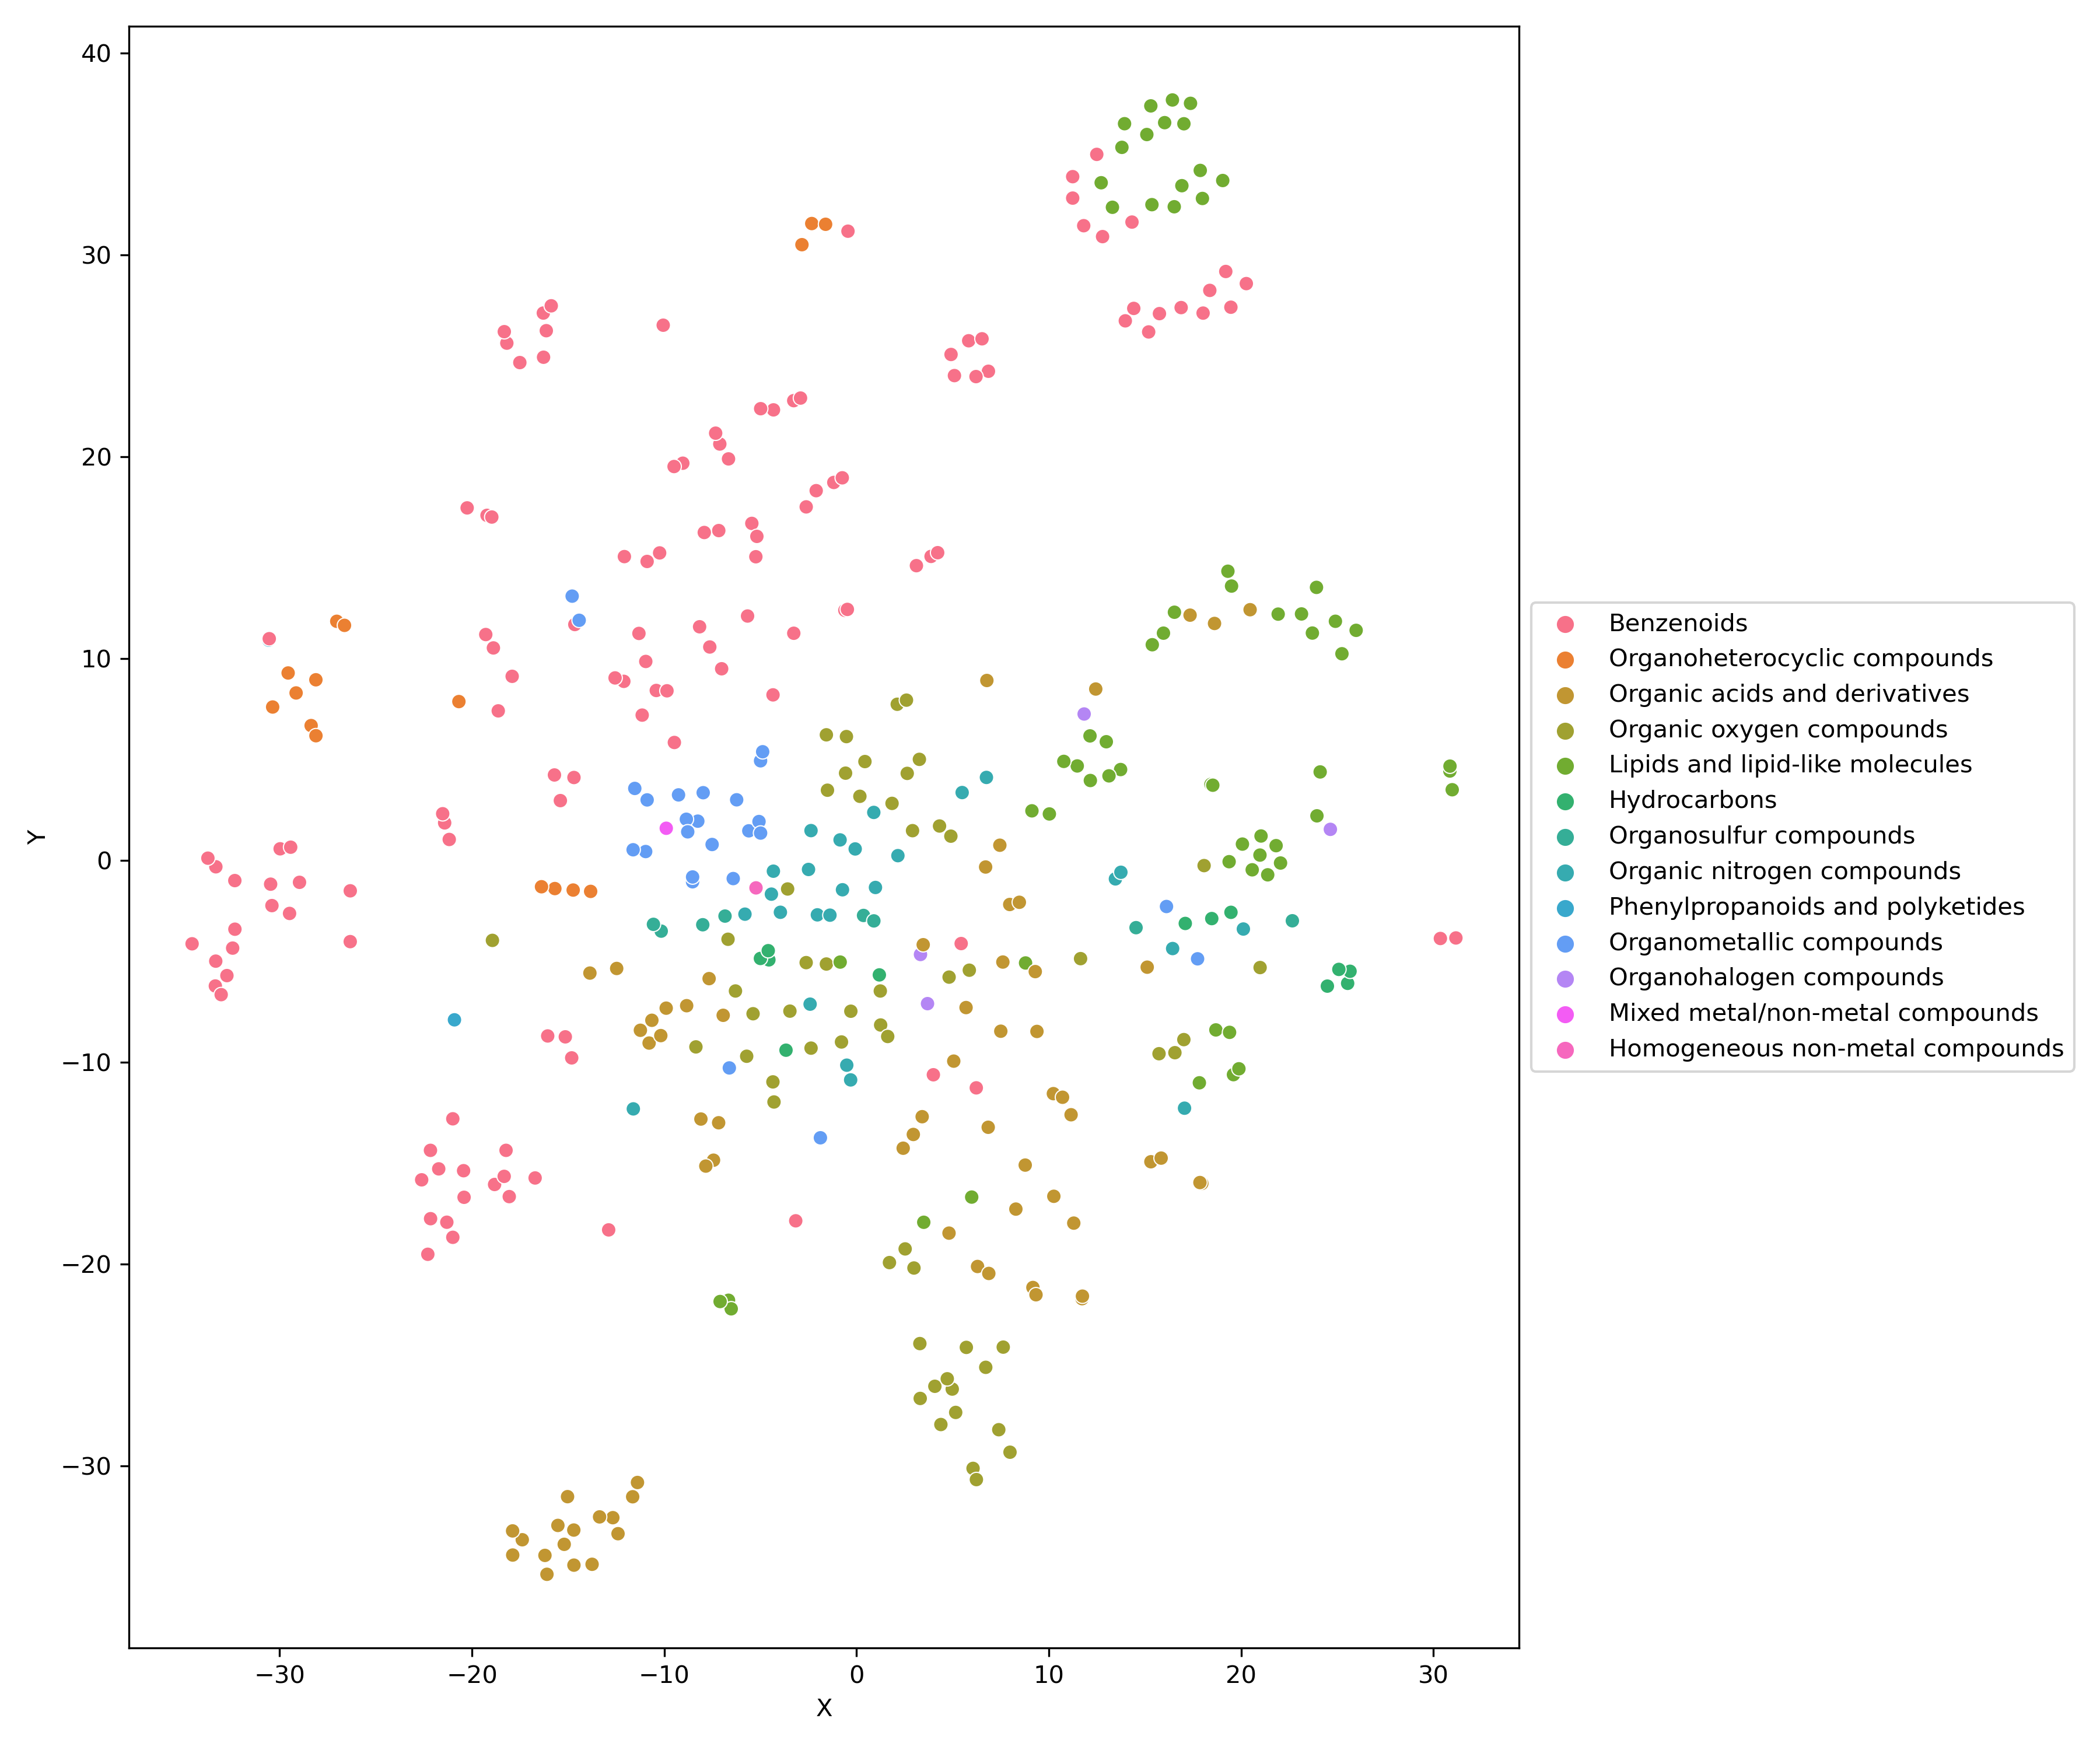
\includegraphics{tsne_df.png} \{\#fig-tsne\}

\subsection{Analogue Evidence Streams}\label{analogue-evidence-streams}

In this study, the analogue identification strategy was recorded for
each read-across case. This was captured in two ways in: 1) a narrative
form and 2) more machine readable manner. The narrative provided a short
description of the way in which analogues were identified and evaluated
for their suitability for reading across the endpoint. The machine
readable summary provided a long pipe-delinated string that captured all
types of similarity rationales used to identify and evaluate analogues.
This was referred to as an ``analogue evidence stream''. An example
would be take the form of
``Structural\_description\textbar Physchem\_description\textbar Metabolism\_description\textbar Mechanistic\_description''.
An actual example is
`Structural\_CHRIP\_OECD-Toolbox\_common-phenolic-group-at-same-position-on-benzotriazole
\textbar{} Physchem\_similar-logKow-volatility \textbar{}
Metabolic\_common-metabolite\textbar Mechanistic\_transcriptomic-profiles\_similar-predicted-MOA
\textbar Toxicity\_common-target-organ'.

To summarise the primary means of identifying candidate source analogues
- the first component of the analogue evidence stream was extracted
which revealed that in 72 cases, structure was the first means of
identifying analogues. In contrast, metabolic similarity was the primary
means of identifying analogues only in 4 cases. Across the 72
structure-based cases, it was possible to summarise the types of tools
and approaches used to identify the candidate analogues. The OECD
Toolbox (www.qsartoolbox.org), the EPA CompTox Chemicals Dashboard
(comptox.epa.gov/dashboard) and ChemIDPlus
(https://pubchem.ncbi.nlm.nih.gov/source/ChemIDplus) or some combination
were the main tools relied upon to identify candidate analogues . The
barplot in \textbf{?@fig-analogue} highlights the main tools and
approaches. Though structural similarity using a similarity metric is
often used by these tools or their combinations, by far the most common
means of identifying structural analogues within the examples was to
look for common scaffolds based on functional groups.

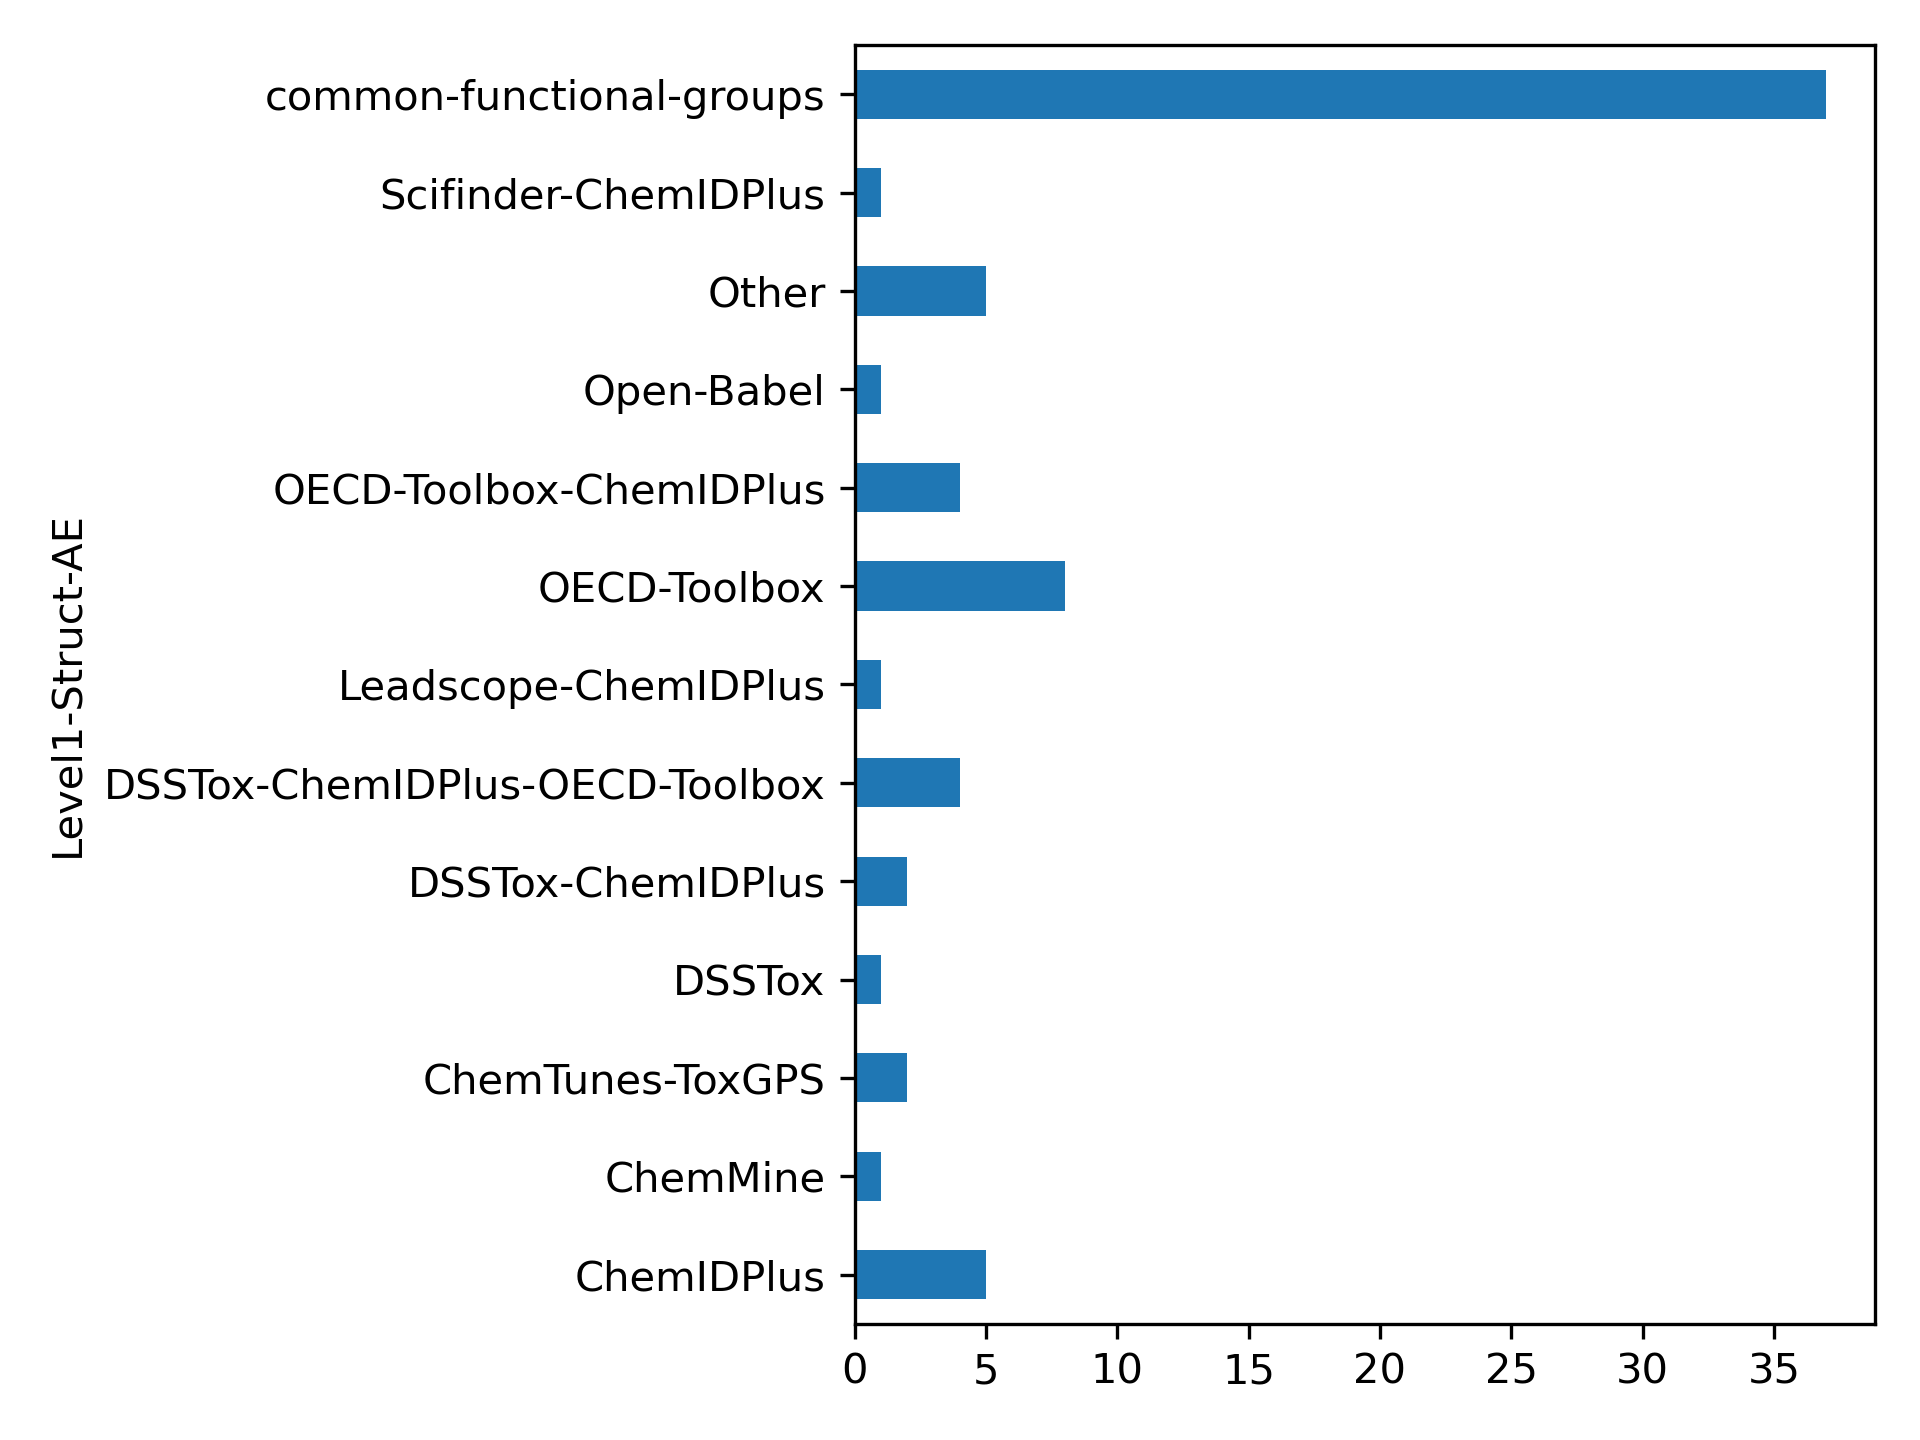
\includegraphics{analogue_stream.png} \{\#fig-analogue\}

\subsection{Similarity contexts}\label{similarity-contexts}

The number of substances per case study varied considerably across the
82 cases with the median number of members being 5 and the maximum
number of members being 42 as shown in \textbf{?@fig-rax}. The size of
these neghbourhoods will have an impact of the range of variation
expected in terms of structural similarity, physicochemical similarity
etc. 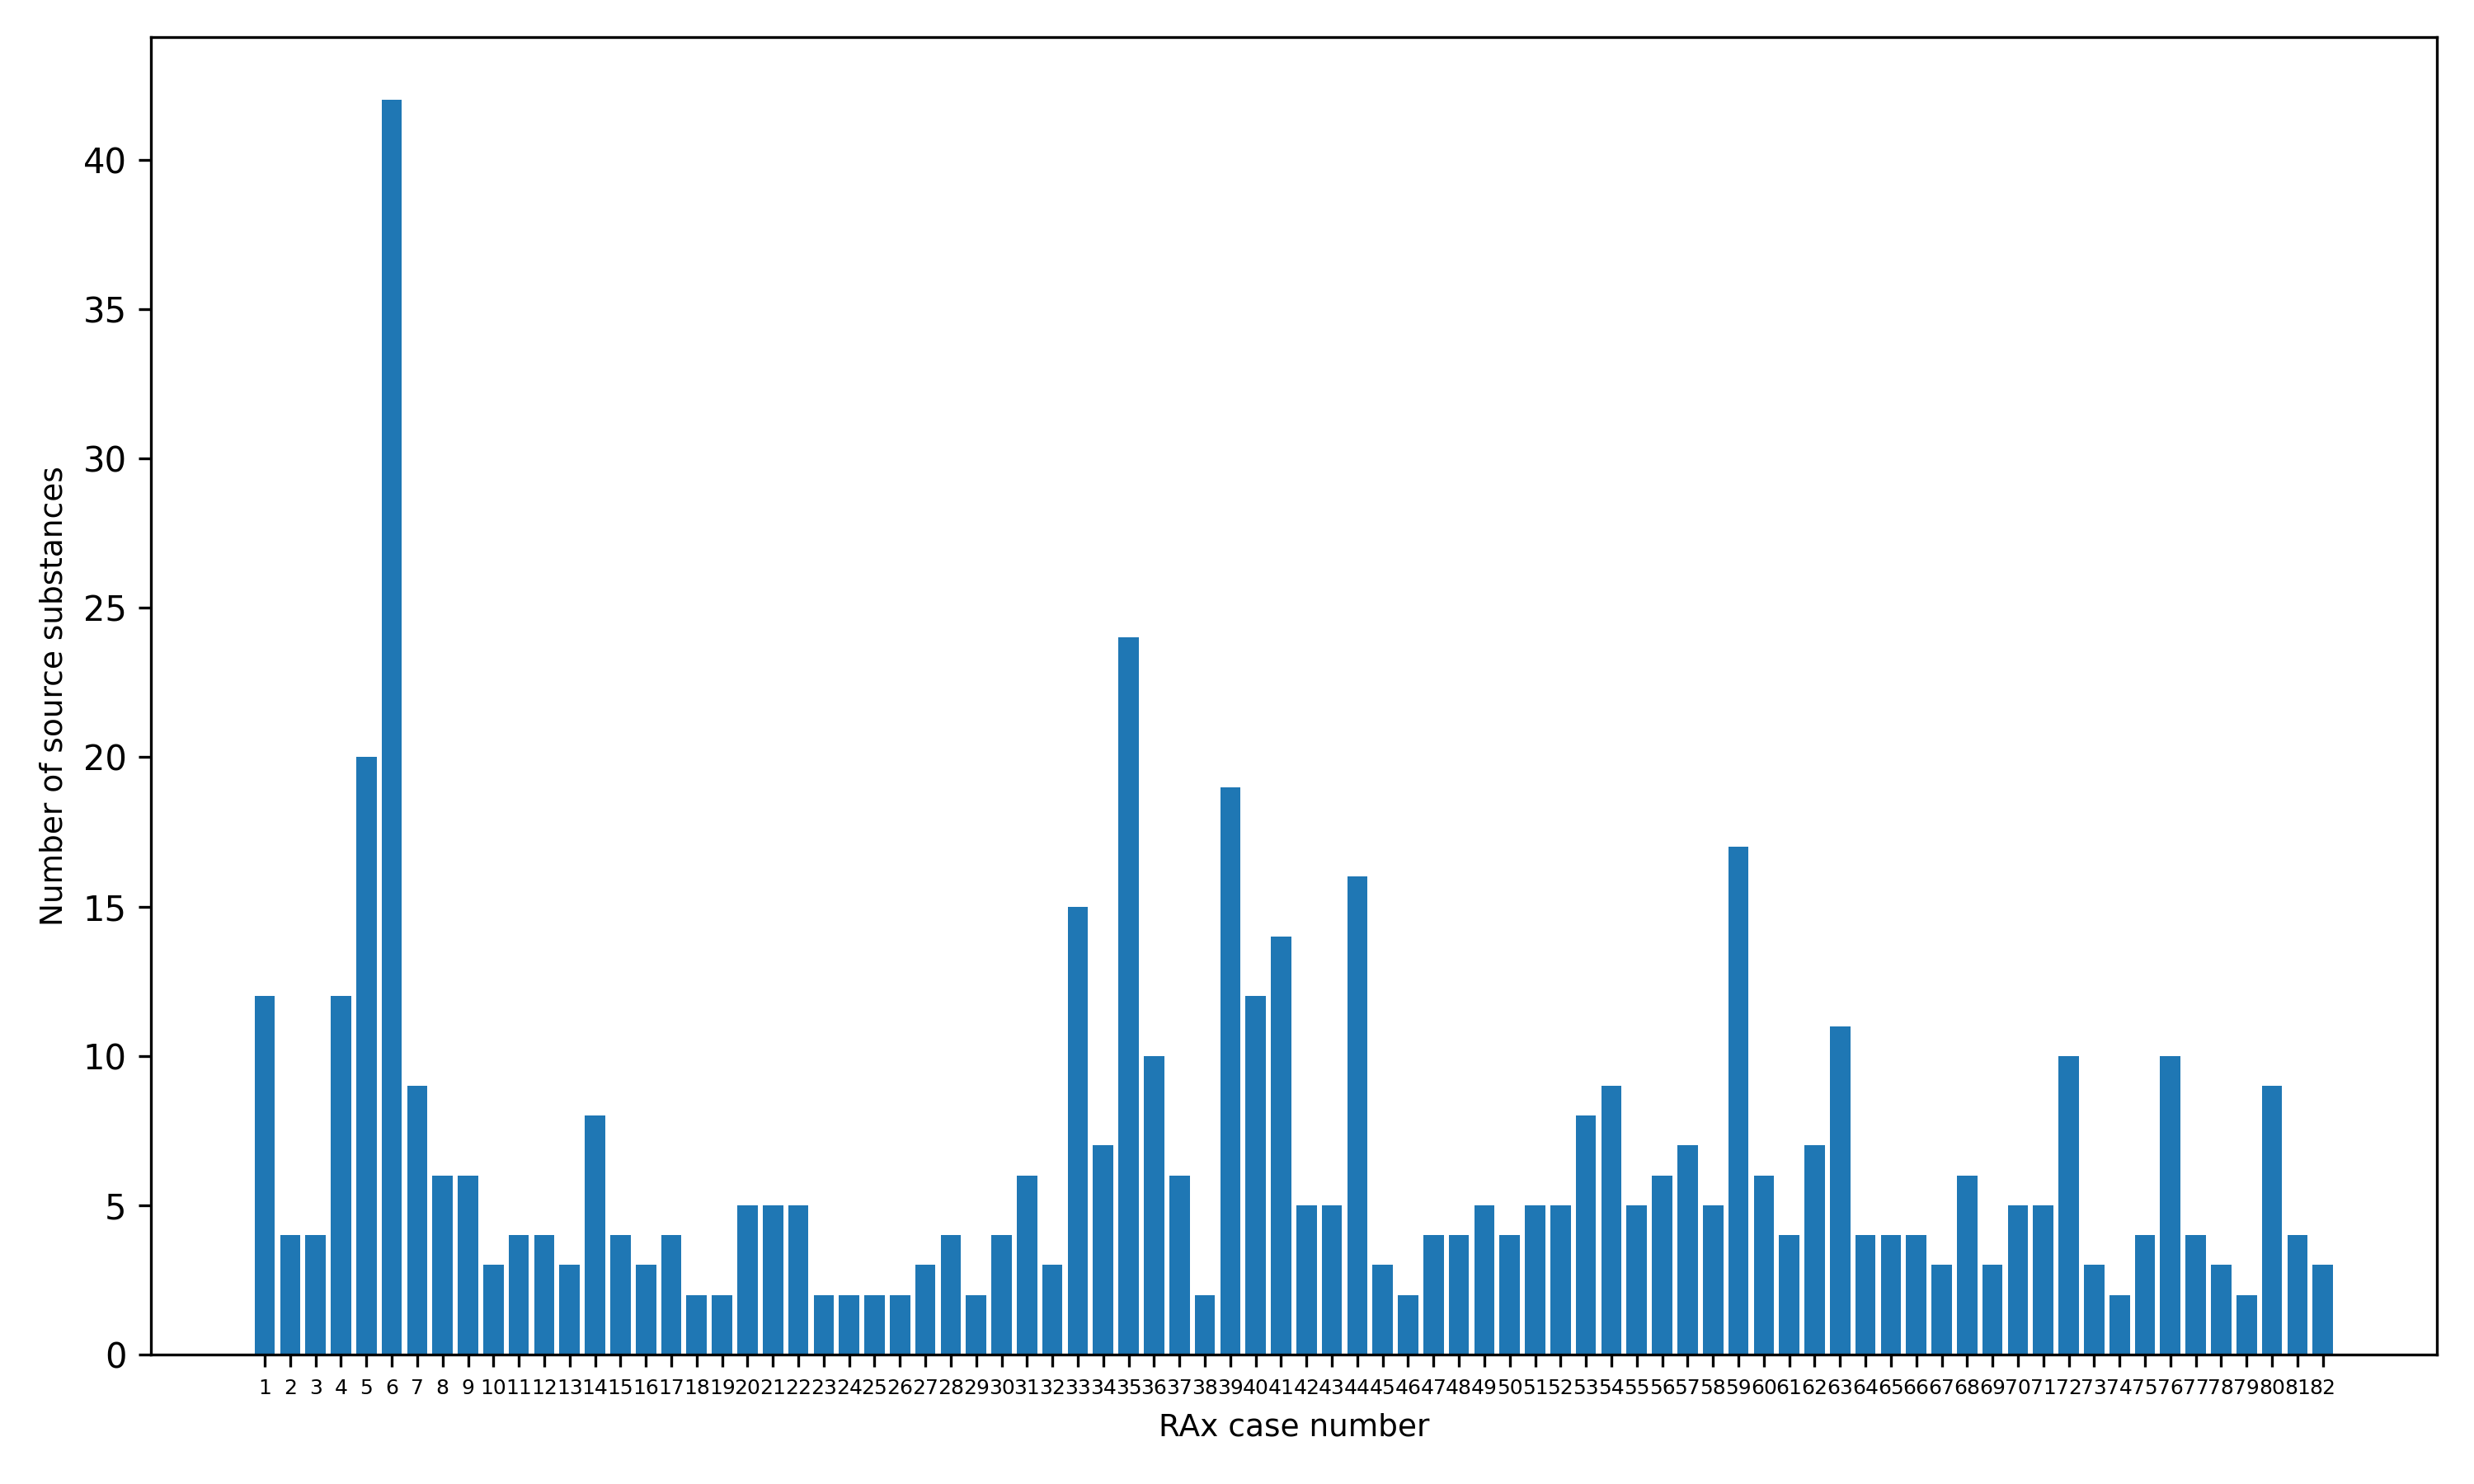
\includegraphics{membership_count.png} \#fig-rax

\subsubsection{Structural similarity
Evaluation}\label{structural-similarity-evaluation}

Pairwise Jaccard structural similarity distributions Figure~\ref{fig-ss}
were computed for all chemicals within each case finding a large
variation in values. Although high Jaccard metrics were observed, the
median of the distribution of median values for each case study was
determined to be only 0.34. \textbf{?@fig-distss} Exploring the
disribution of Jaccard structural similarities within each case also
showed a large degree of variation (See \textbf{?@fig-boxplotss}).

\begin{figure}

\begin{minipage}{0.50\linewidth}

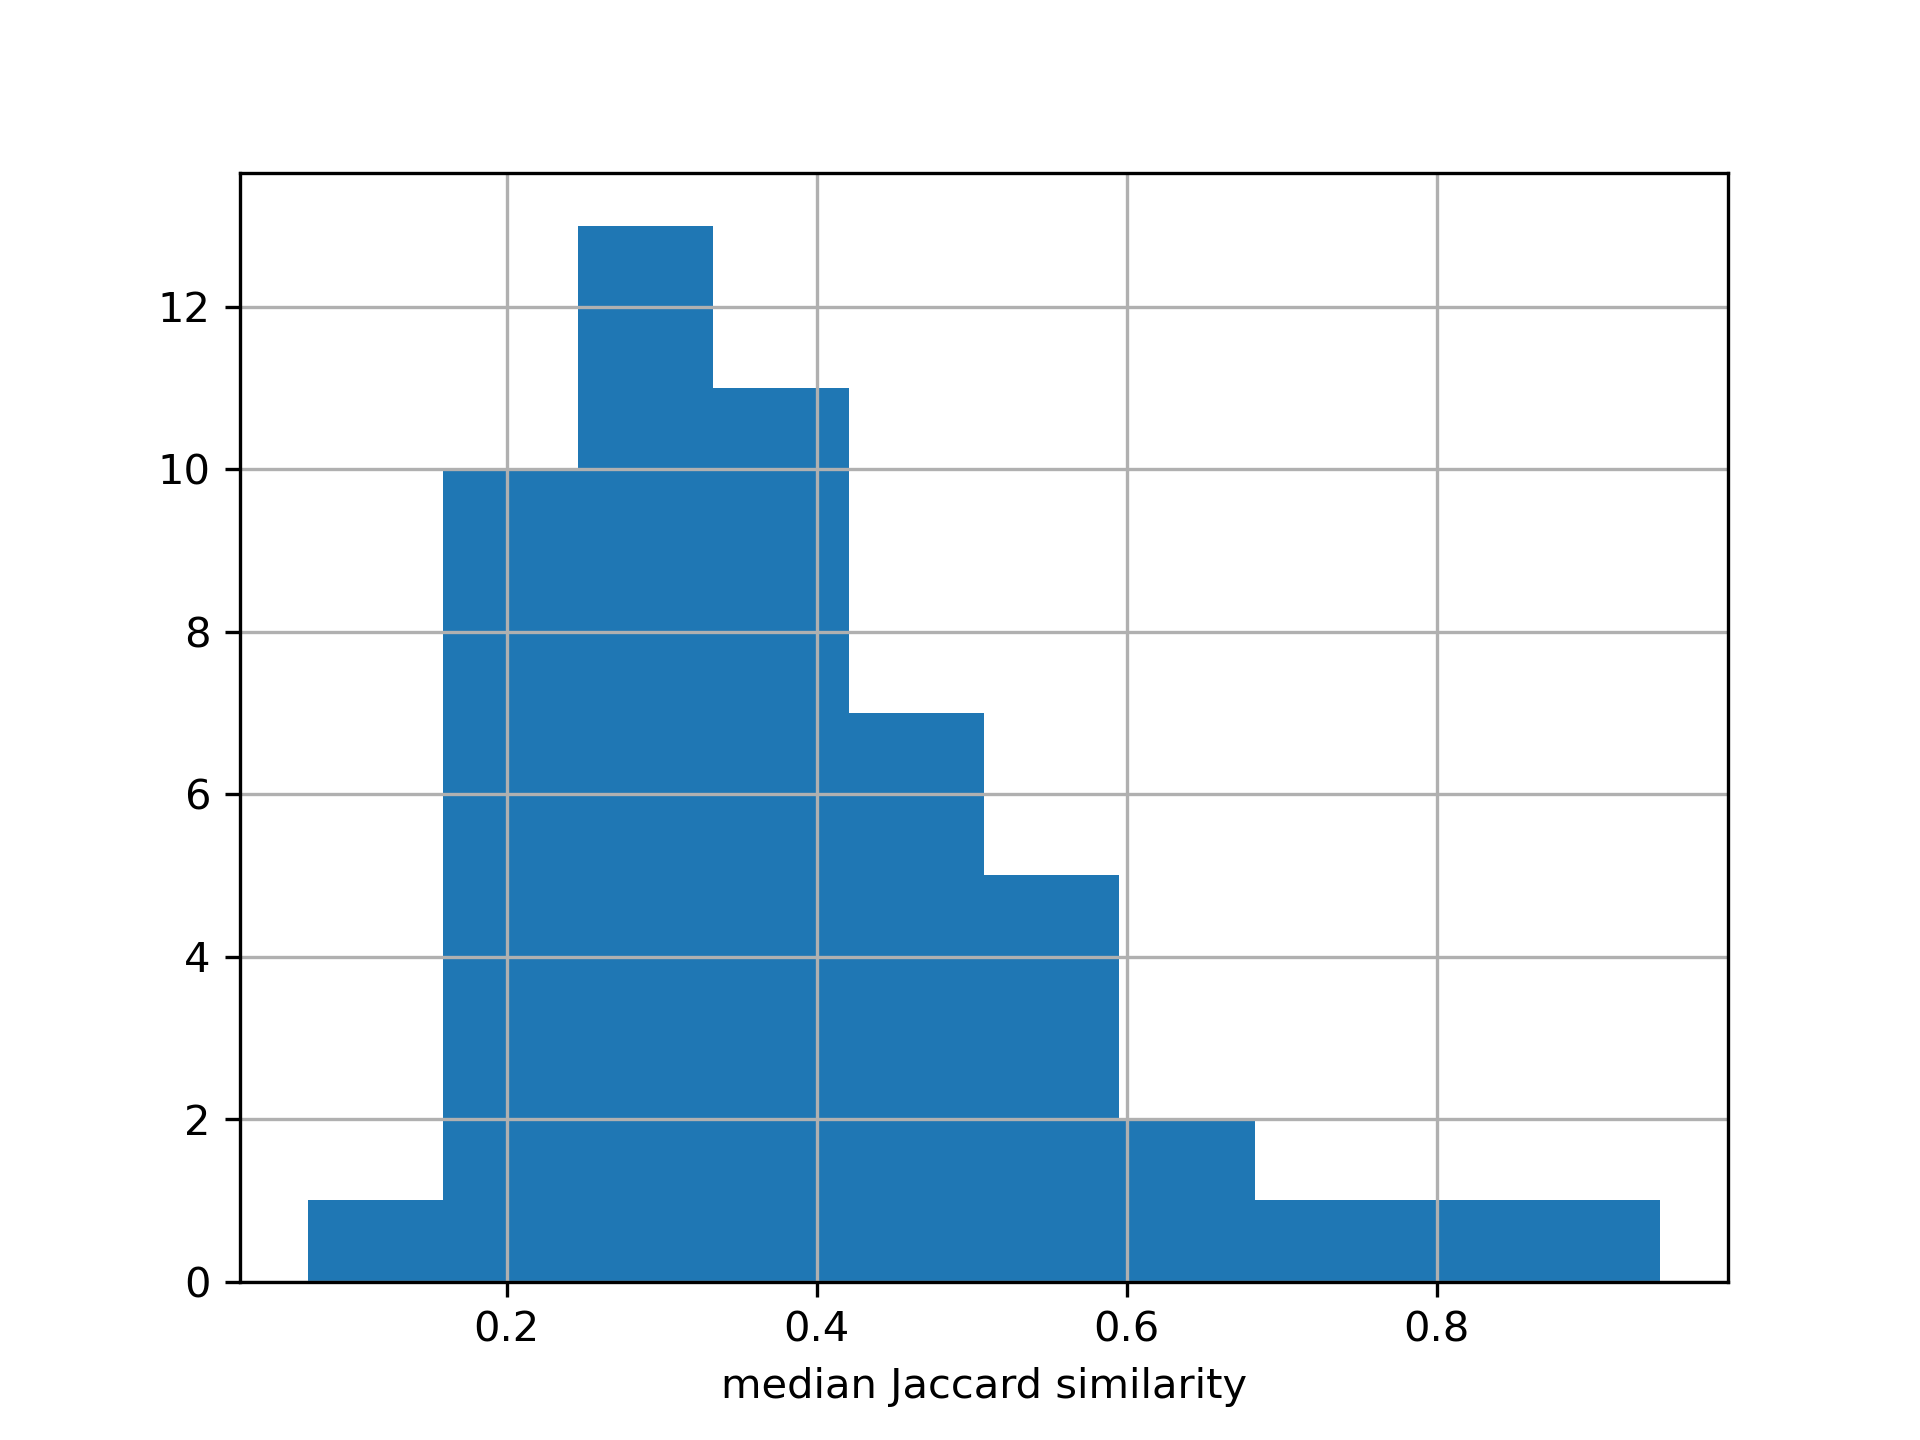
\includegraphics{median_JS_dist.png}

\end{minipage}%

\end{figure}%

\subsection{Alert Similarity
Evaluation}\label{alert-similarity-evaluation}

There were 69 unique endpoint-toxicophore combinations across the
substances included in the read-across cases. This captured 30 specific
endpoints ranging from bone marrow toxicity, irritation to chromosomal
damage and kidney function-related toxicity. A pairwise comparison of
the profile across these endpoint-toxicophore combinations either was
not particularly informative - substances either showed complete or no
overlap, the same variation was noted within each read-across case as
shown in \textbf{?@fig-alert}. A similar pattern of variation in
physicochemical similarity within each read-across case was also seen in
\textbf{?@fig-phys}.

\begin{figure}

\begin{minipage}{0.50\linewidth}

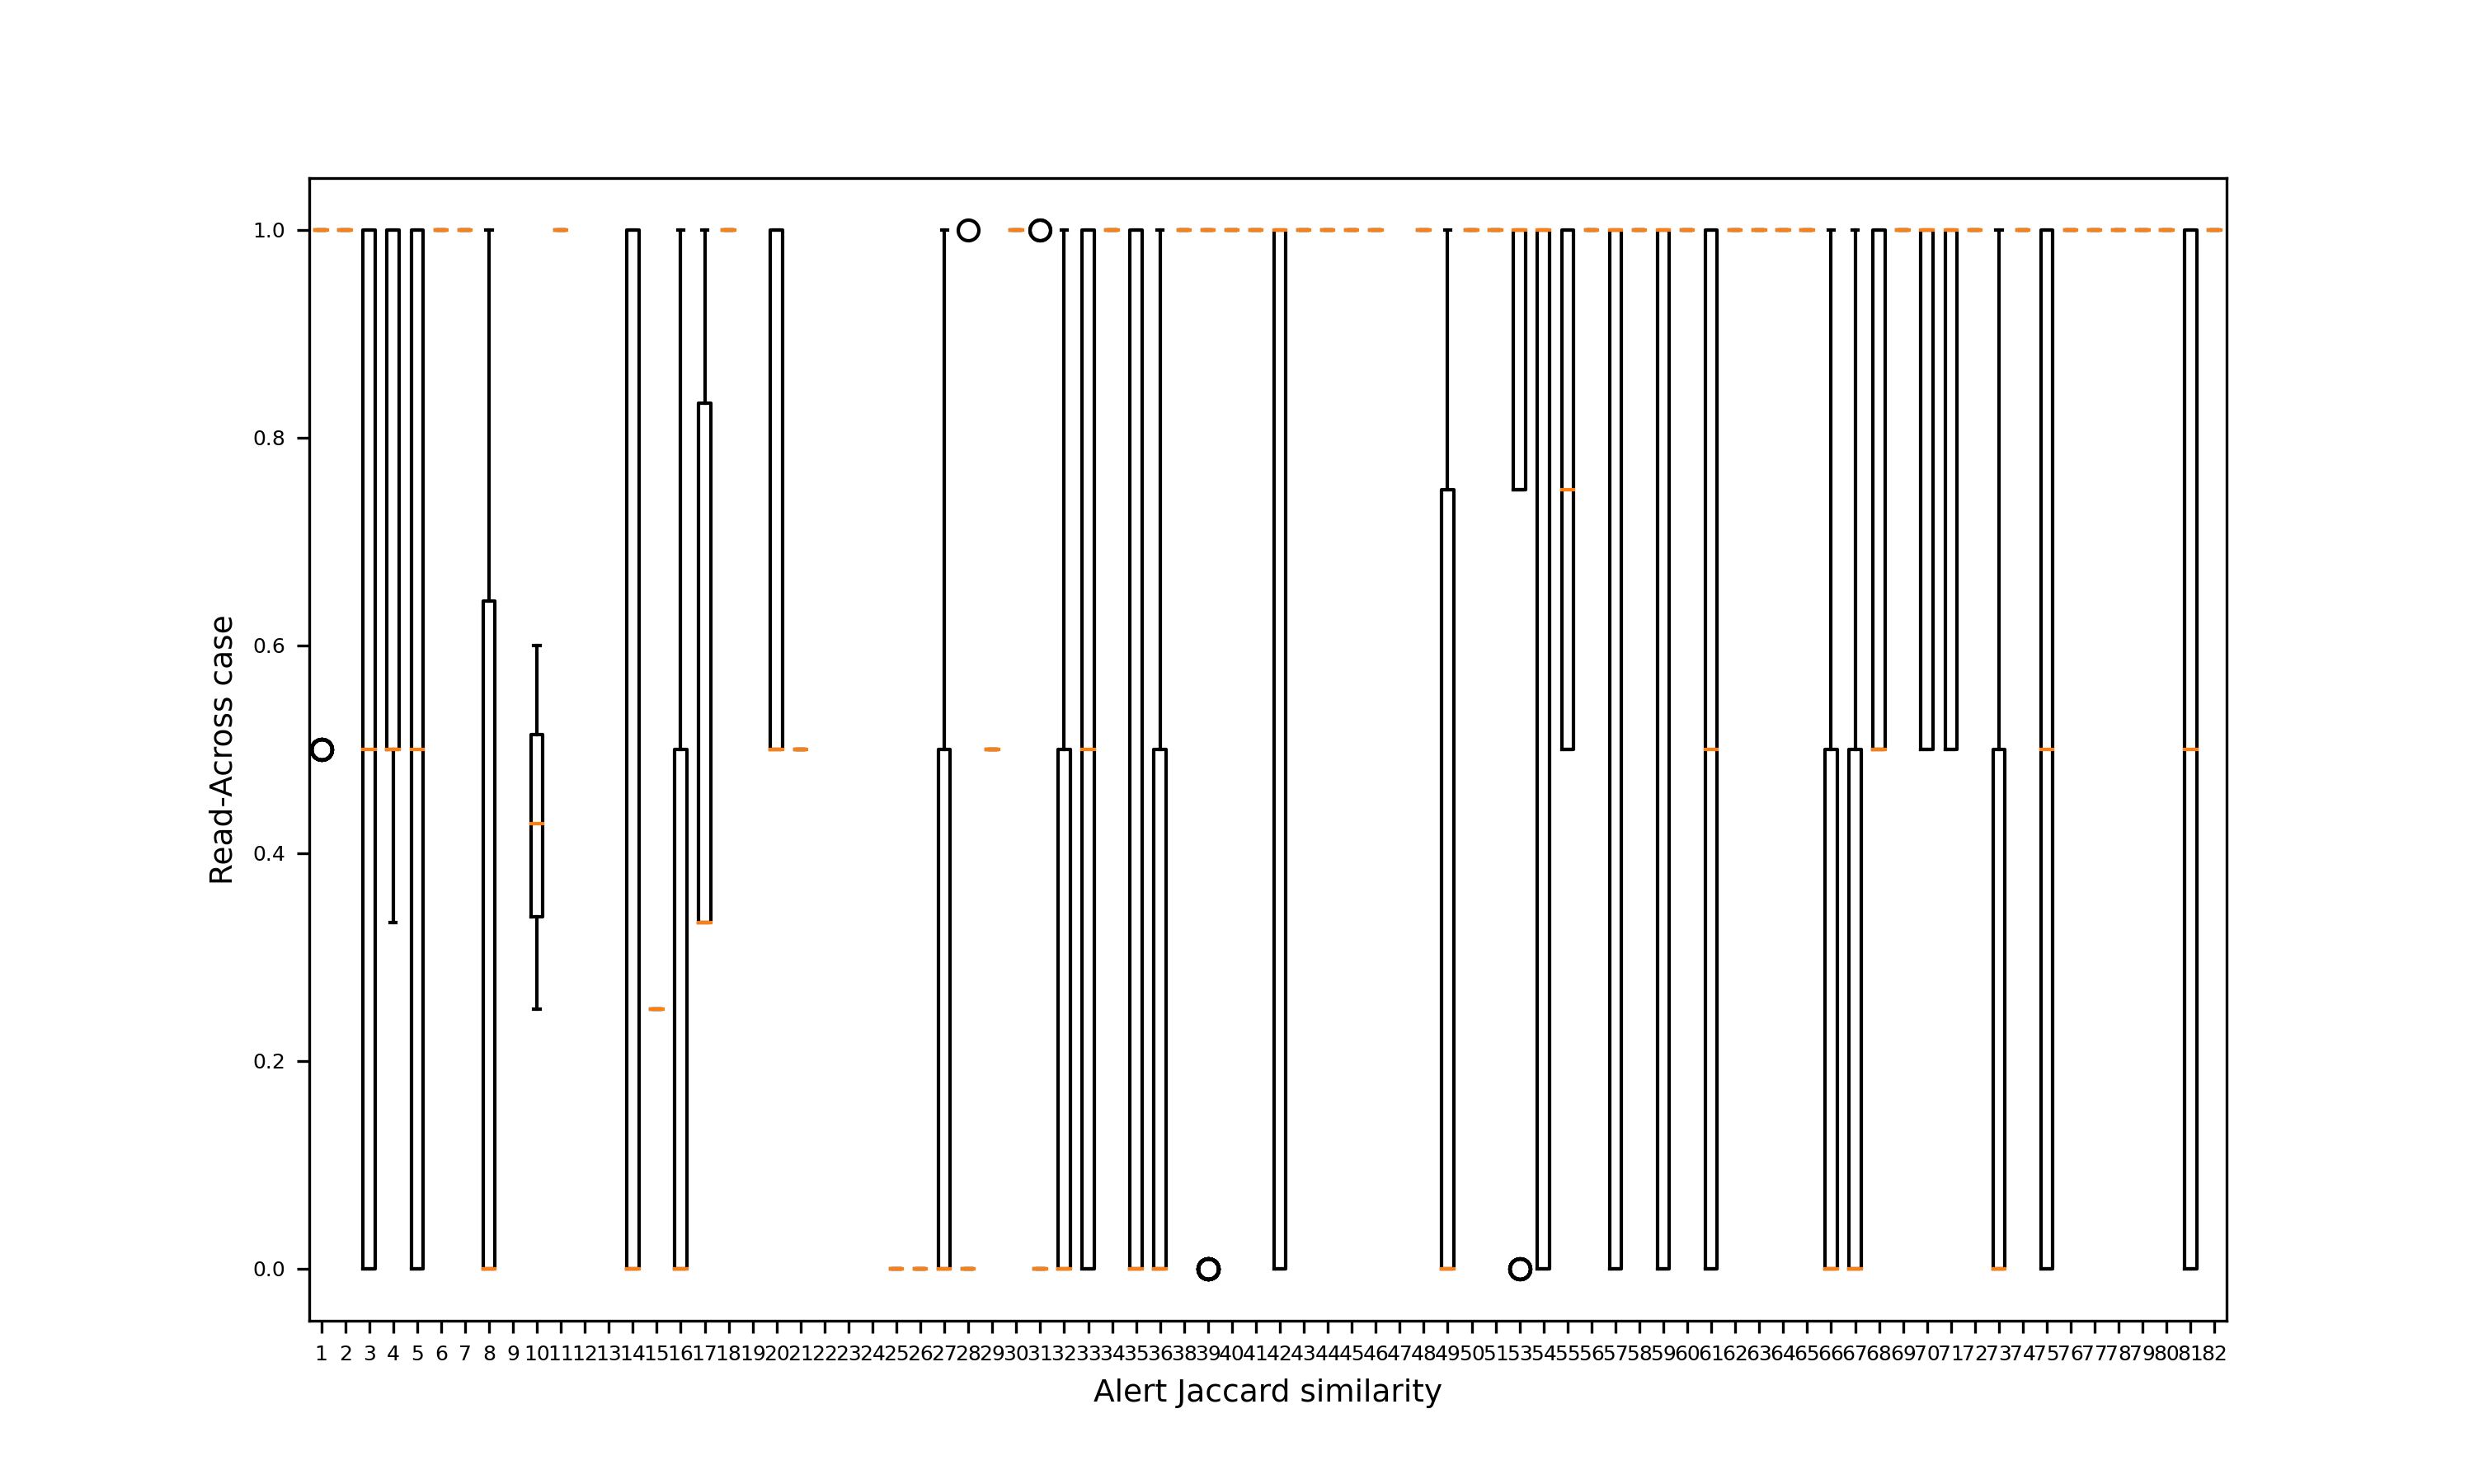
\includegraphics{Alert_similarity.png}

\end{minipage}%

\end{figure}%

\subsubsection{Metabolic Similarity
Evaluation}\label{metabolic-similarity-evaluation}

The pairwise similarities were computed within each read-across example
to explore how metabolically similar the target and source analogues
were amongst themselves with respect to their metabolic graph
Figure~\ref{fig-wl}, transformation profile Figure~\ref{fig-trans} and
metabolites \textbf{?@fig-mets} as shown in Figure~\ref{fig-ms} There
was a large degree of variation in pairwise similarities within each
case study and the similarities were low overall.

\begin{figure}

\begin{minipage}{0.33\linewidth}
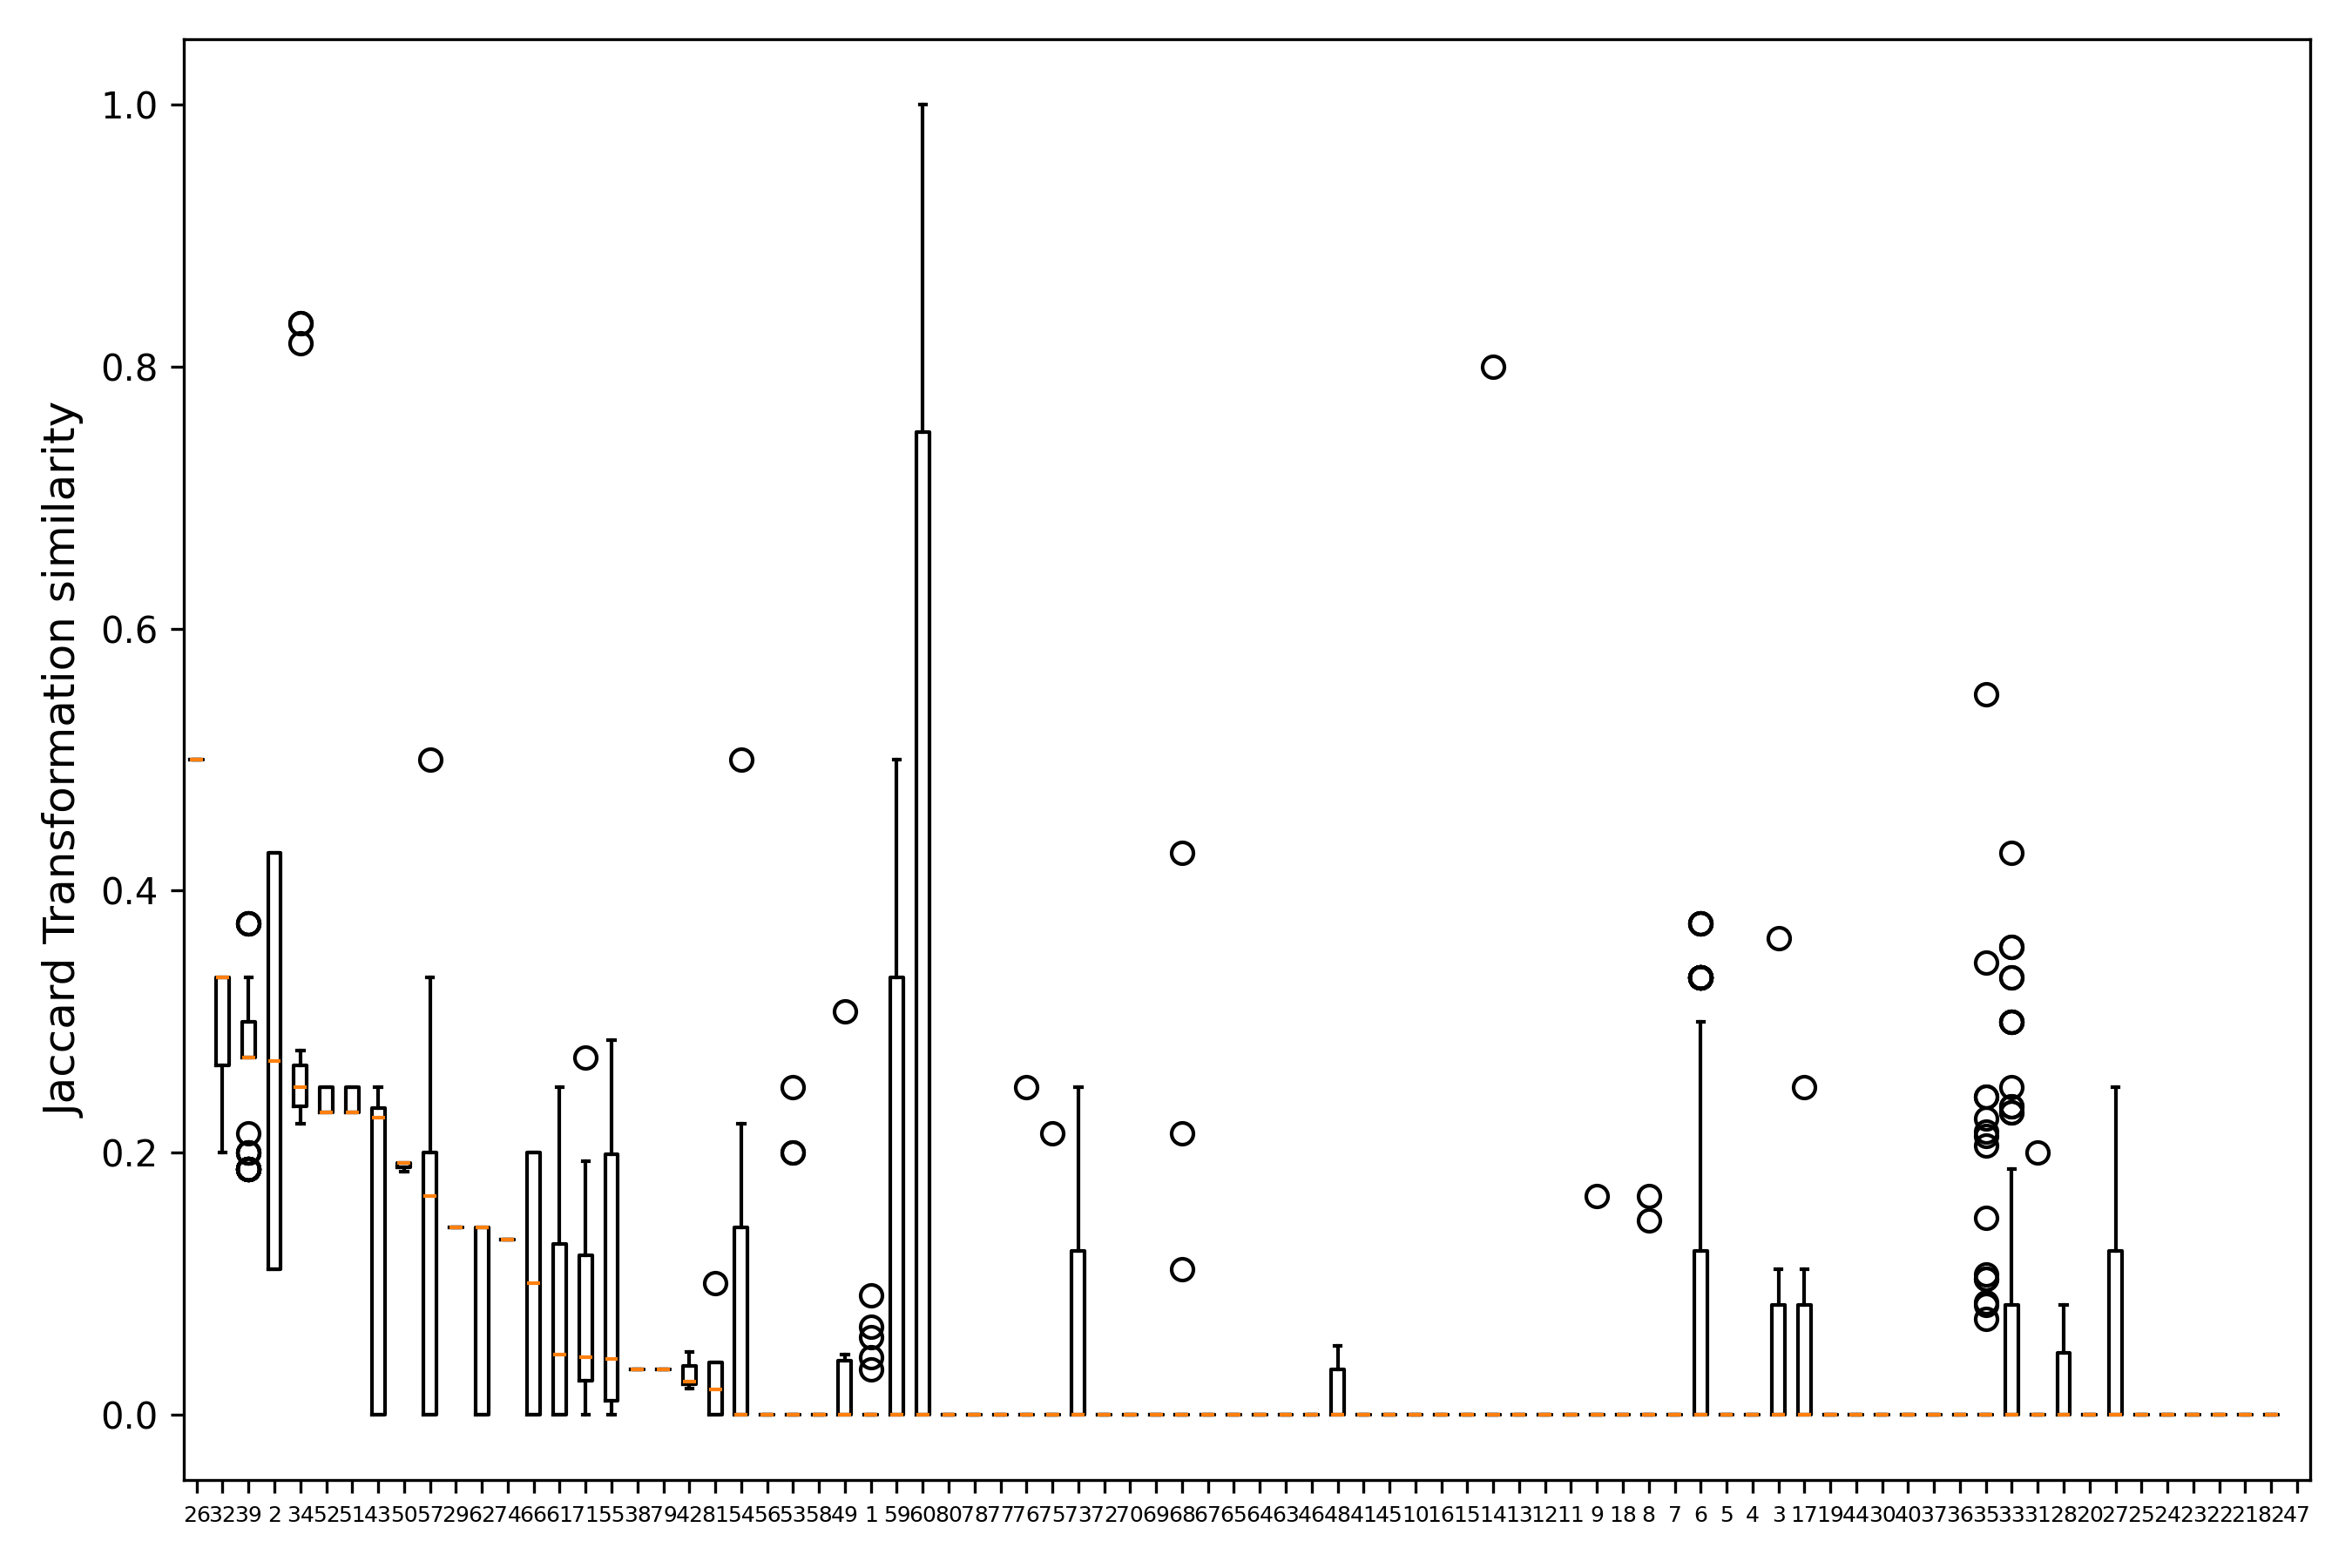
\includegraphics{Jaccard_metabolites_similarity_200124.png} \{\#fig-mets
width=``50\%''\}\end{minipage}%
%
\begin{minipage}{0.33\linewidth}

\centering{

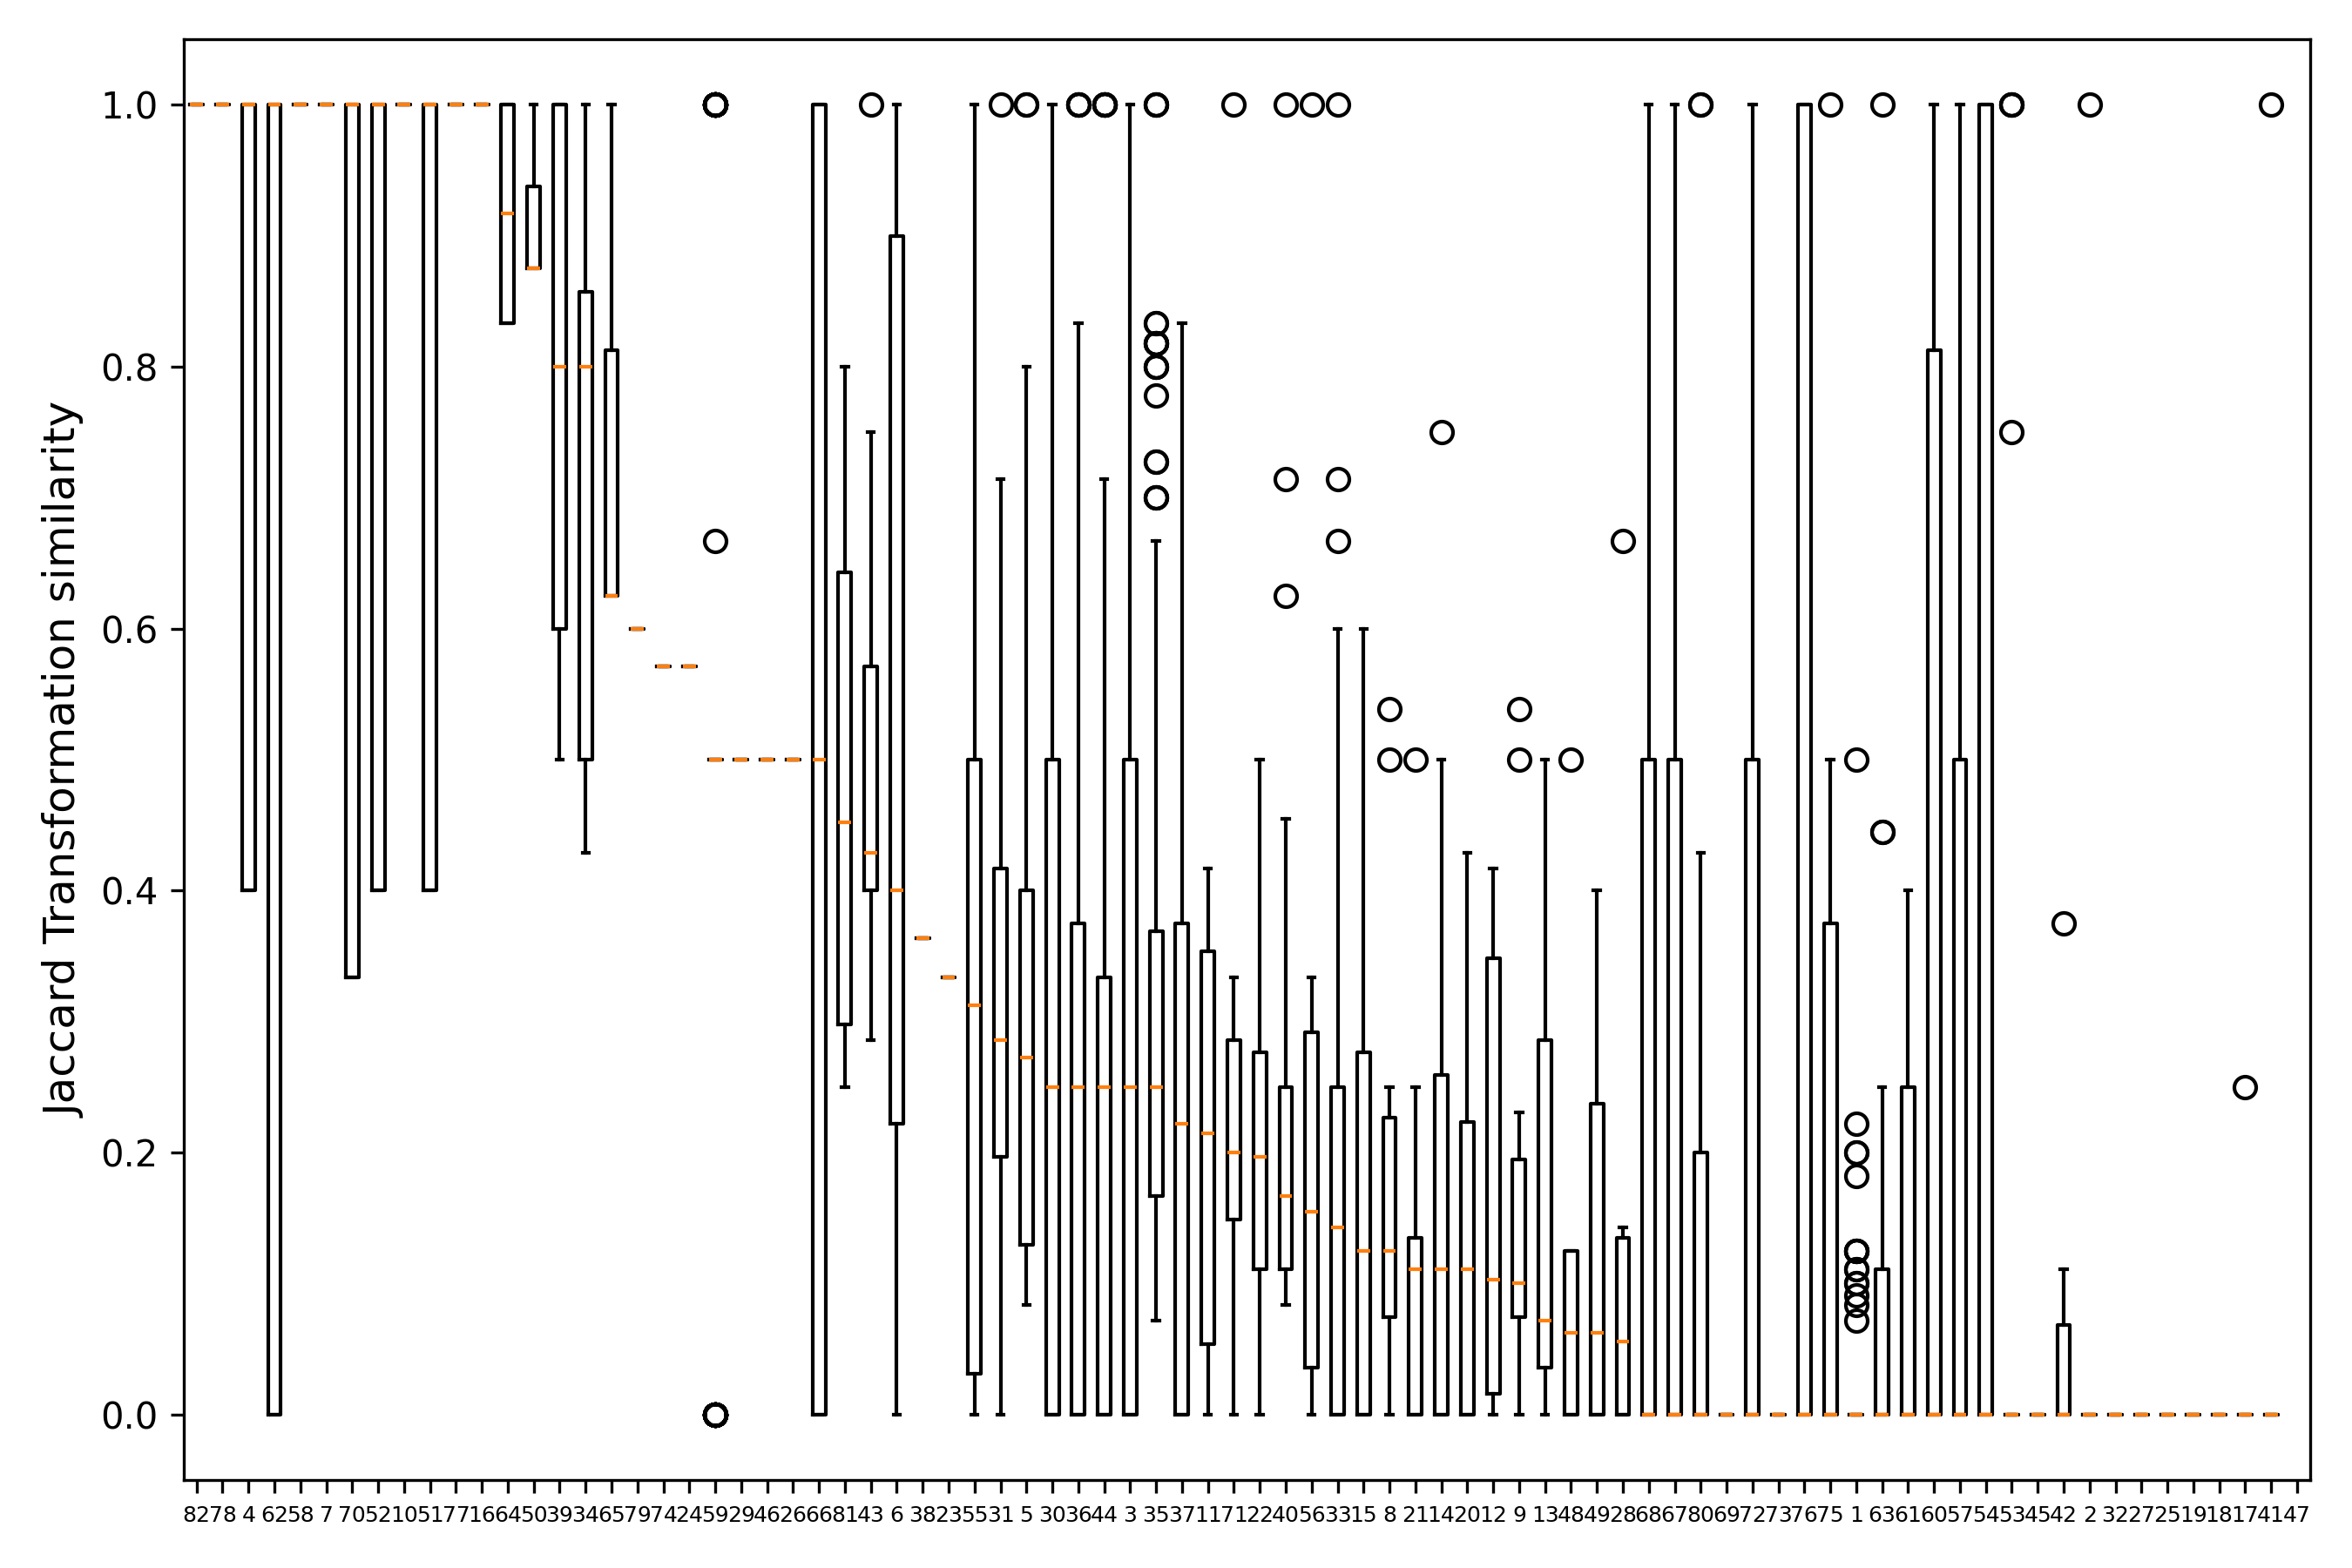
\includegraphics[width=0.5\textwidth,height=\textheight]{Jaccard_transformation_similarity_200124.png}

}

\subcaption{\label{fig-trans}Boxplot of pairwise Jaccard transformation
similarities within each read-across example}

\end{minipage}%
%
\begin{minipage}{0.33\linewidth}

\centering{

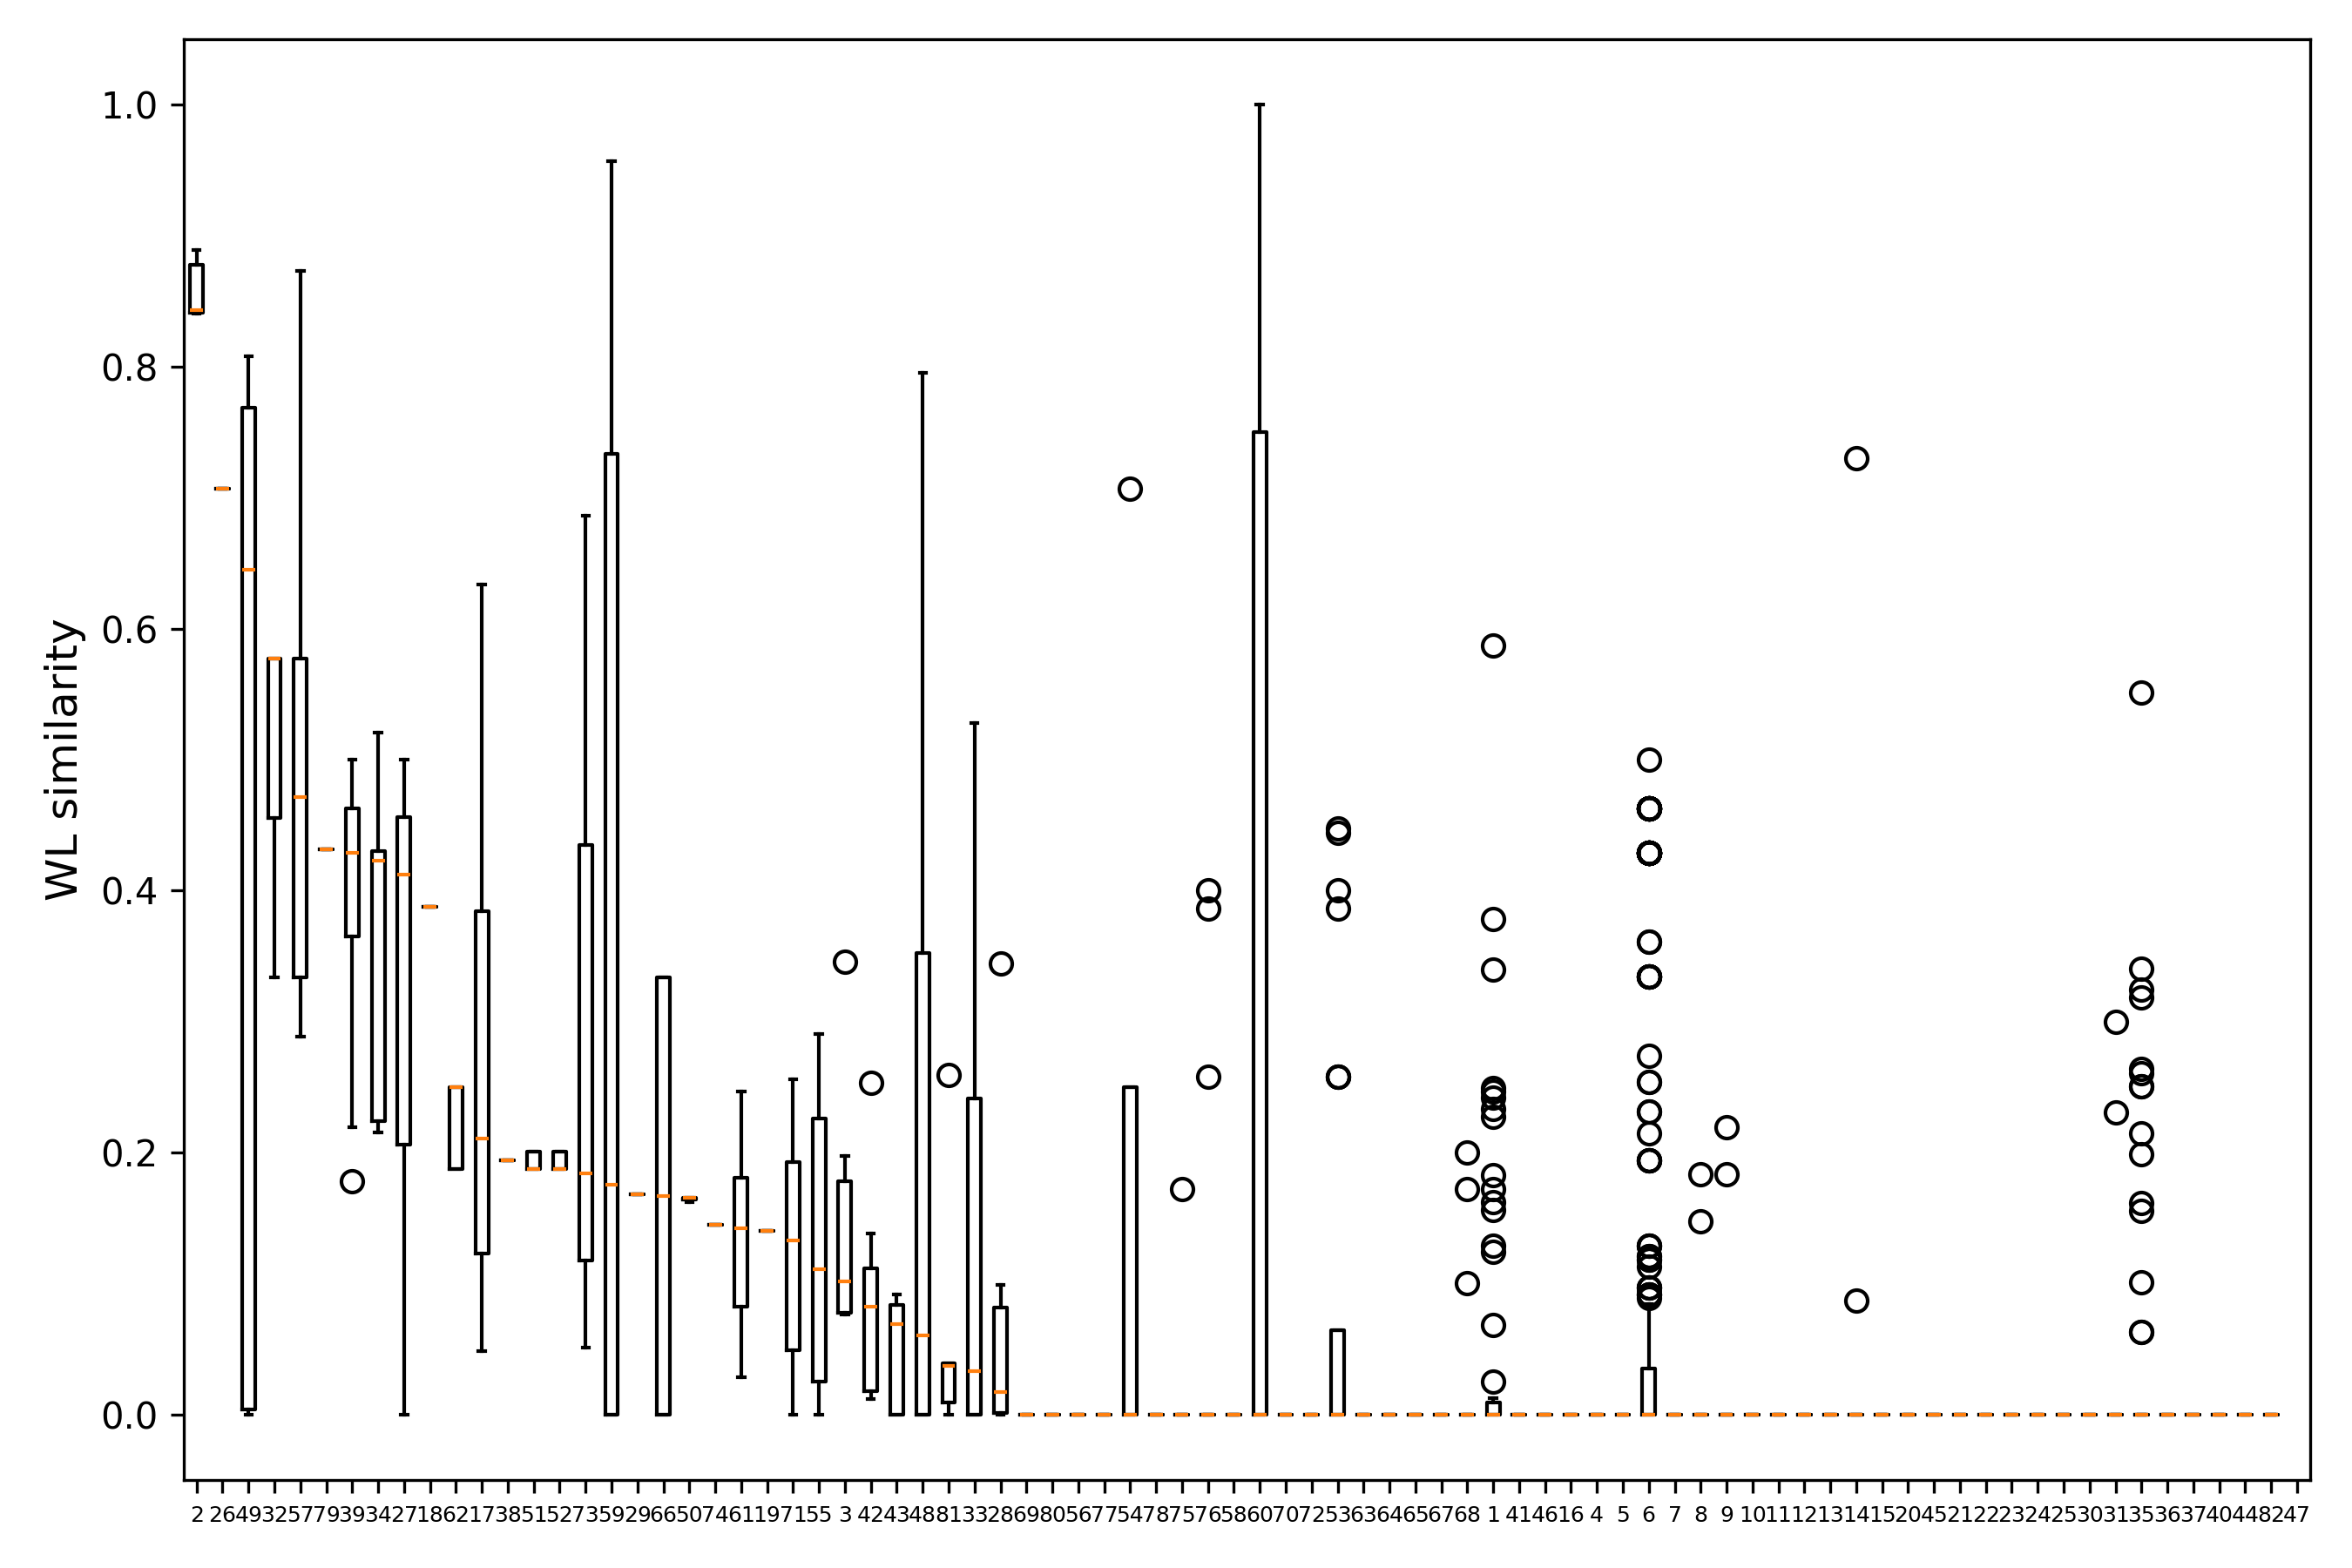
\includegraphics[width=0.5\textwidth,height=\textheight]{WL_similarity_200124.png}

}

\subcaption{\label{fig-wl}Boxplot of pairwise WL graph kernel
similarities within each read-across example}

\end{minipage}%

\end{figure}%

\subsection{Bayesian Logistic Regression of the balanced labelled
analogue
pairs}\label{bayesian-logistic-regression-of-the-balanced-labelled-analogue-pairs}

4 chains converged and the Rhat across the parameters all successfully
converged. Based on the trace summary the similarity metric with the
highest contribution for whether a pair of substances were similar was
structural similarity, followed by similarity in the metabolism based on
the graph kernel and transformation pathway. \textbf{?@fig-pp} shows the
posterior plot for the parameters estimated. The greatest uncertainty
arises in the similarity of the metabolites. The balanced accuracy of
the test set was determined to be 0.83. \textbf{?@fig-cm} shows the
confusion matrix for the test set predictions using the mean parameters.
The profile of the parameters is well aligned to the features found to
be most pertinent in the Patlewicz et al (2024) study even though the
dataset was larger and more diverse.

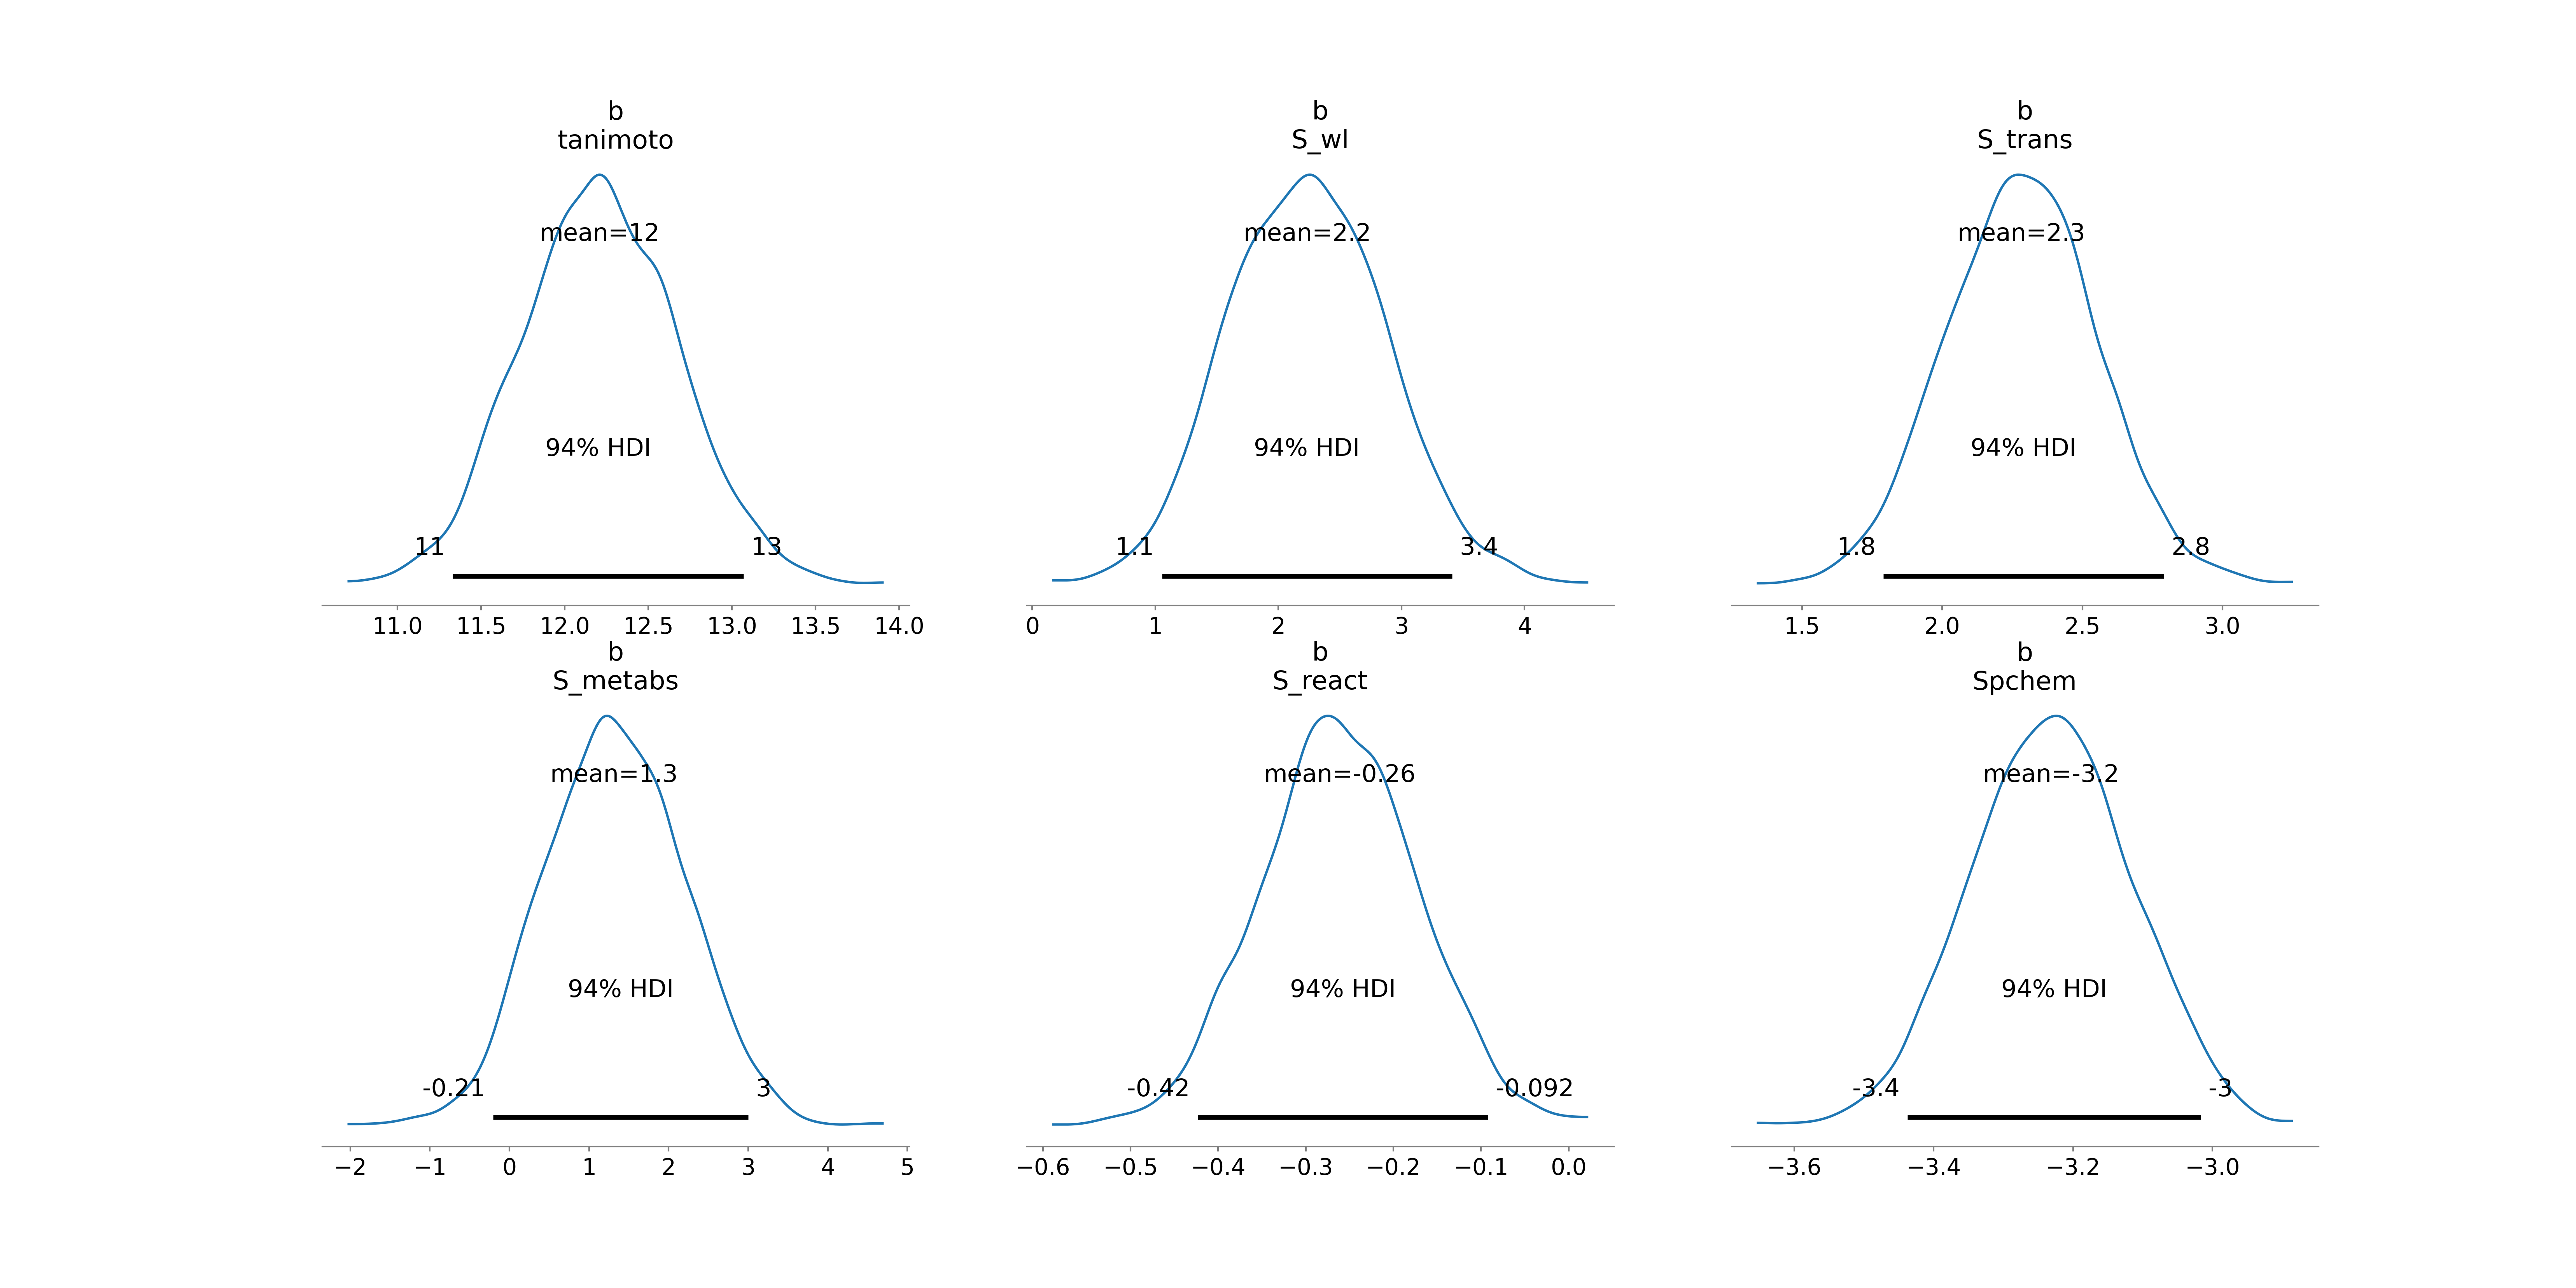
\includegraphics{posterior_plot.png} \{\#fig-pp width=``50\%''\}

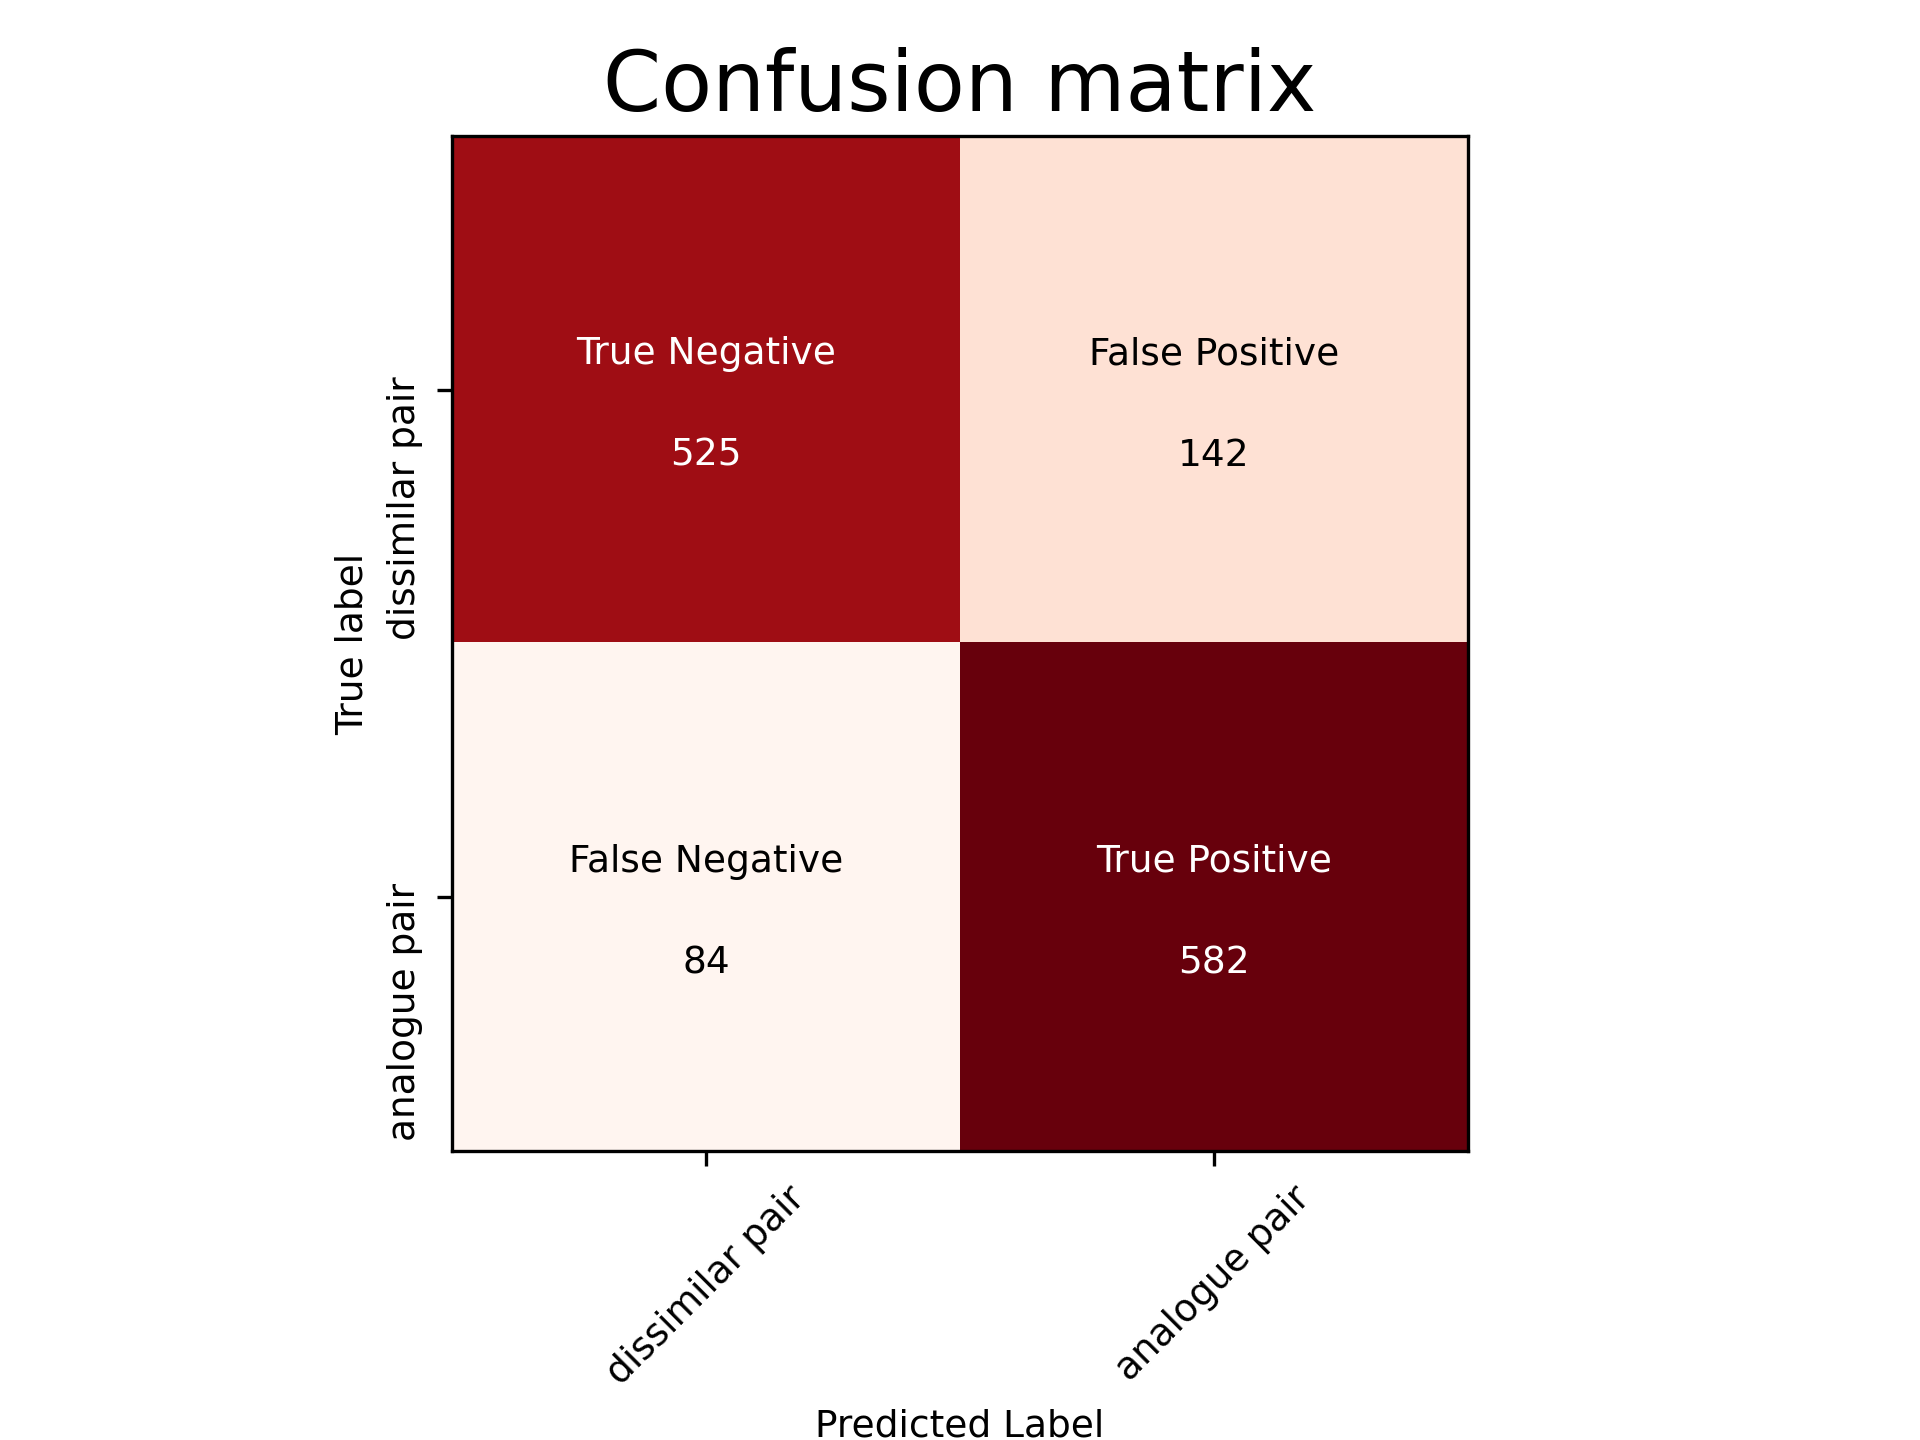
\includegraphics{confusion_matrix.png} \{\#fig-cm width=``50\%''\}

\subsection{Deep learning approach}\label{deep-learning-approach}

The deep learning approach using pytorch objects constructed from the
SMILES themselves with the Graph Isomerism Approach network failed to
create embeddings which could discriminate between similar and
dissimilar analogue pairs. Whilst the accuracy was 0.67, the precision,
recall and F1 scores on the test set were respectively 0.89, 0.40 0.55.
Similarly the Graph Convolutional Network failed to create
discriminating embeddings. The accuracy was only 0.6 with a precision,
recall and F1 score of 0.68, 0.34 and 0.45 respectively.

\subsection{Shallow learning approach}\label{shallow-learning-approach}

Using the same balanced dataset constructed, an ITML approach was
performed as part of a stratified 5-fold CV workflow. The mean CV
balanced accuracy was found to be 0.95 (sd 0.0058). A grid search for
the hyperparameter gamma found that 0.75 gave rise to the highest mean
CV performance. The ITML model was refit on the training set and
predictions were made on the test set that had not been used during the
training and testing loops. The accuracy of the test set was 0.95.

\subsection{UMAP}\label{umap-1}

Using the same balanced dataset constructed, a supervised UMAP was
applied to learn an embedding that could discriminate similar pairs from
dissimilar pairs. Different neighbours were used to preserve local
structure in the emdeddings though 5 neighbours proved to show the best
separation in 2D for training and test sets Figure~\ref{fig-umap}.

\begin{figure}

\begin{minipage}{0.50\linewidth}

\centering{

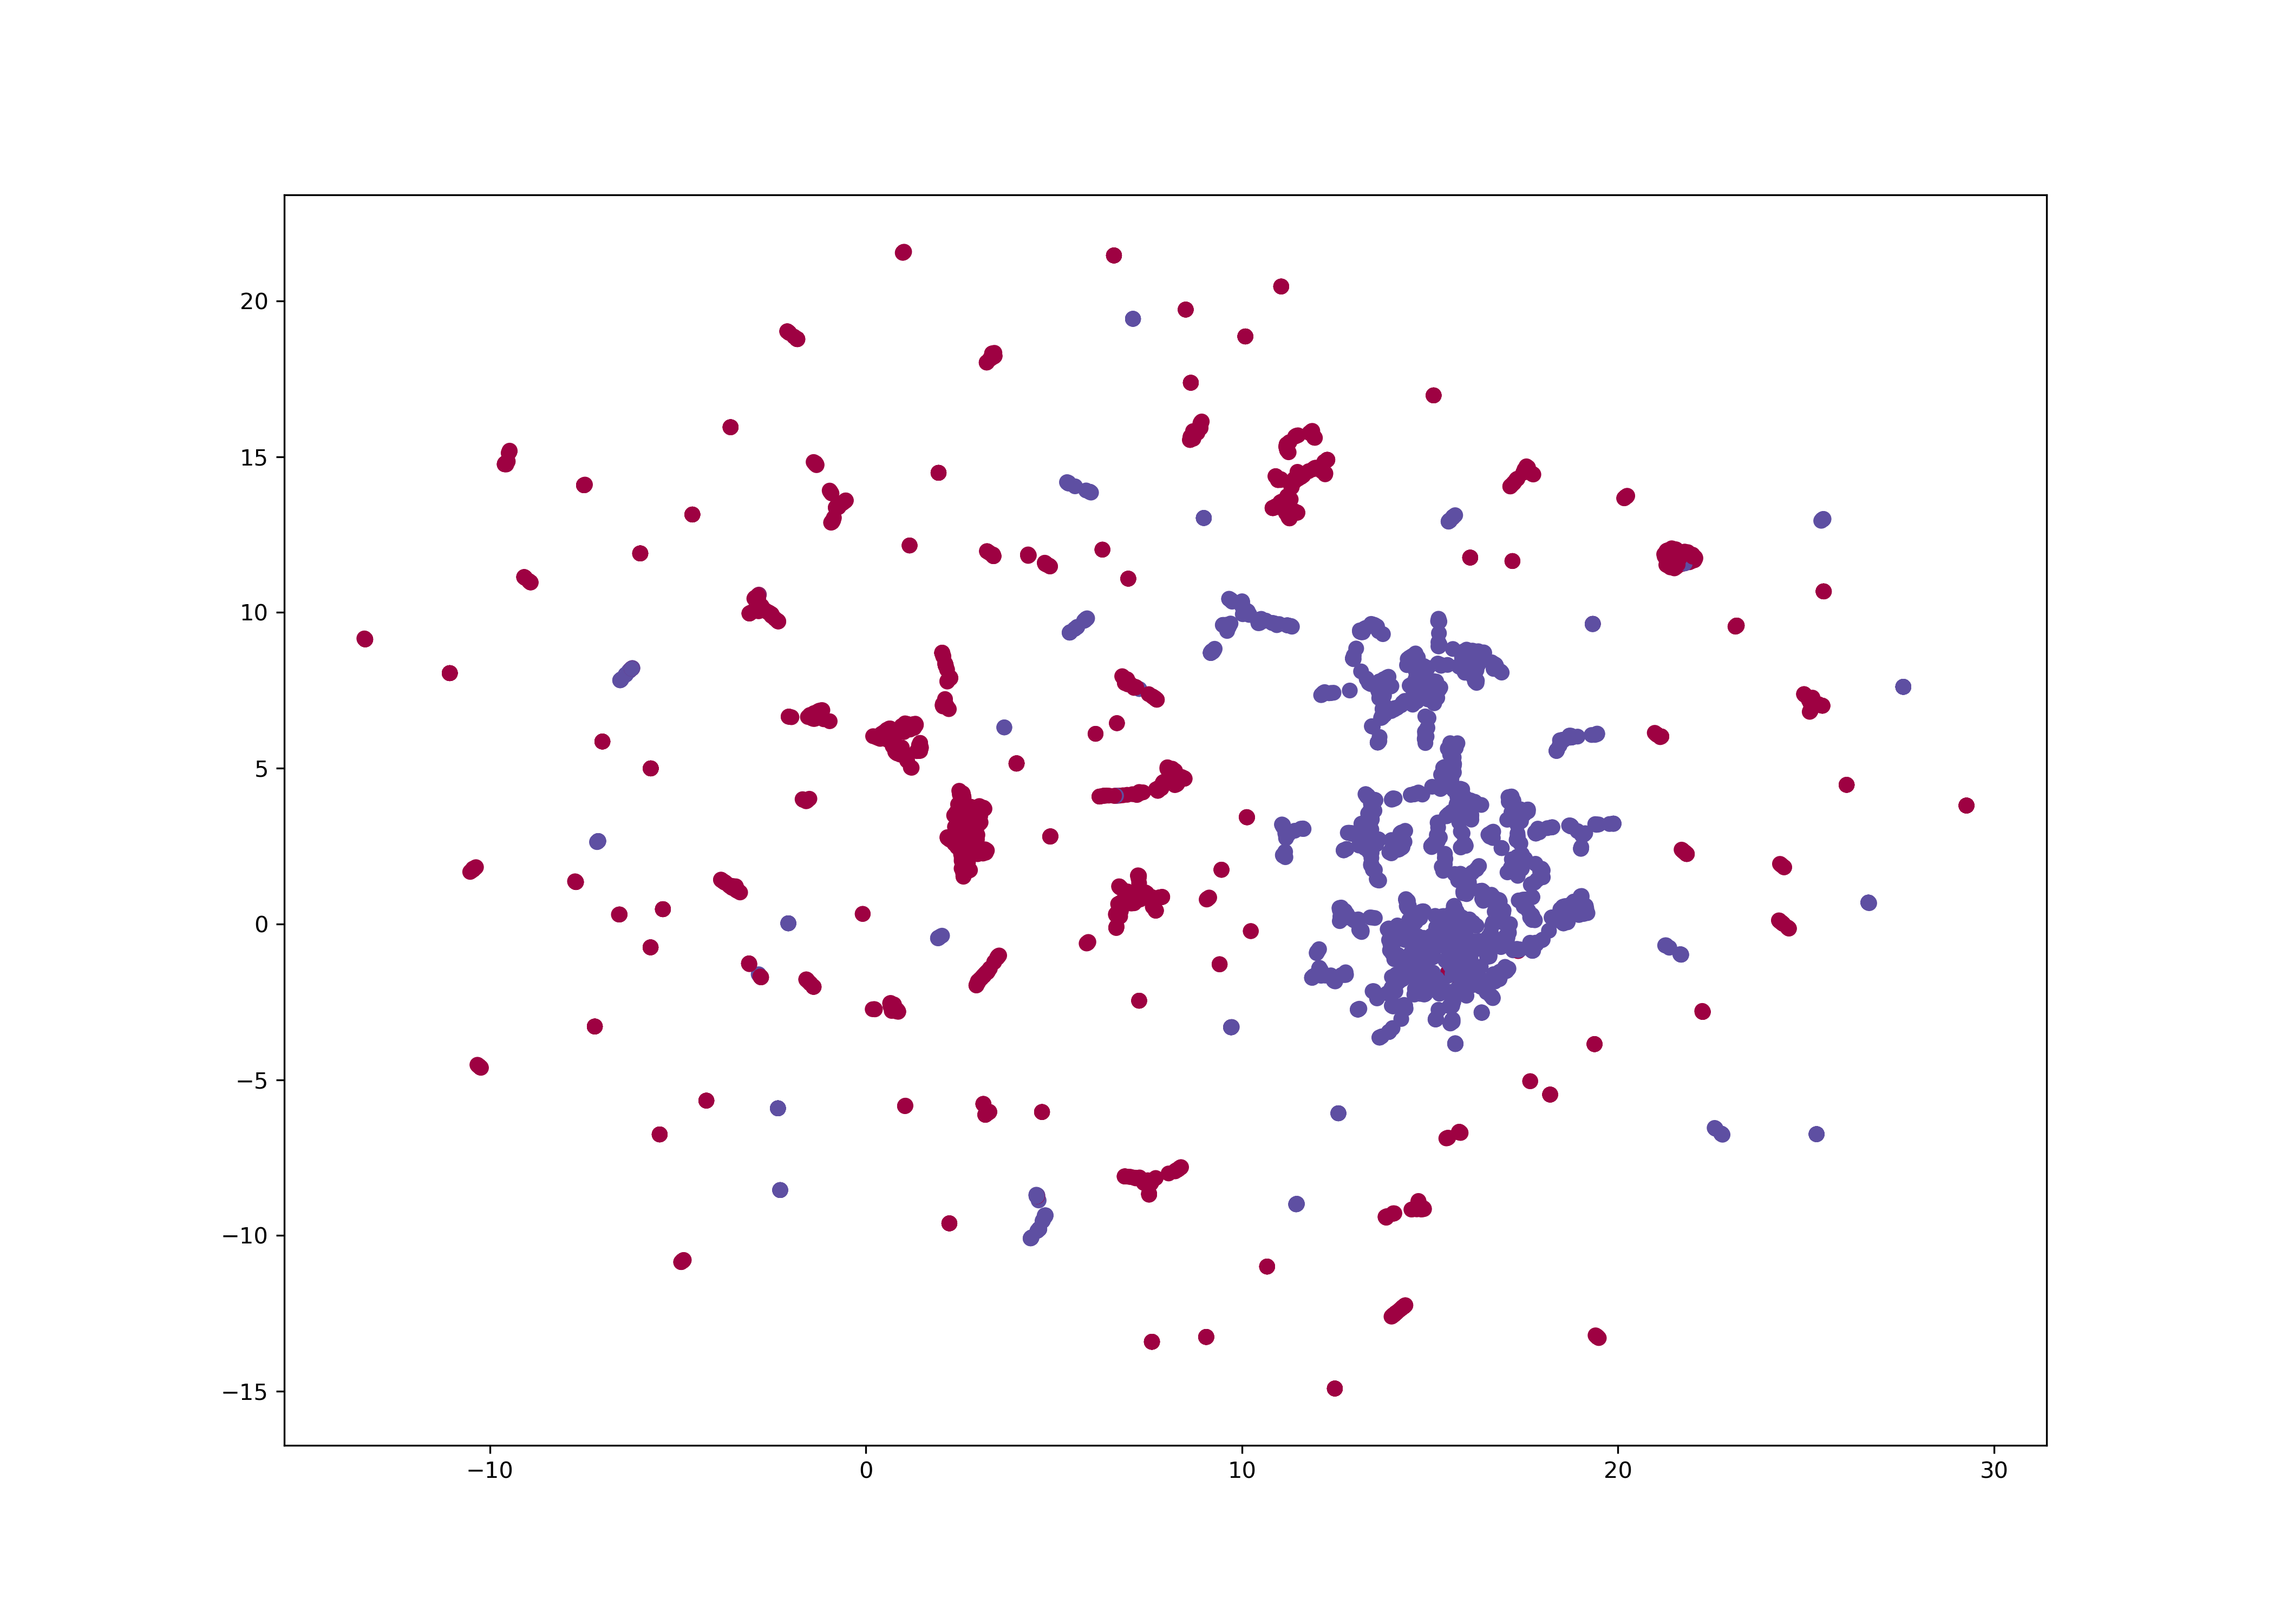
\includegraphics[width=0.5\textwidth,height=\textheight]{train_embedding.png}

}

\subcaption{\label{fig-umaptrain}Supervised UMAP training set}

\end{minipage}%
%
\begin{minipage}{0.50\linewidth}

\centering{

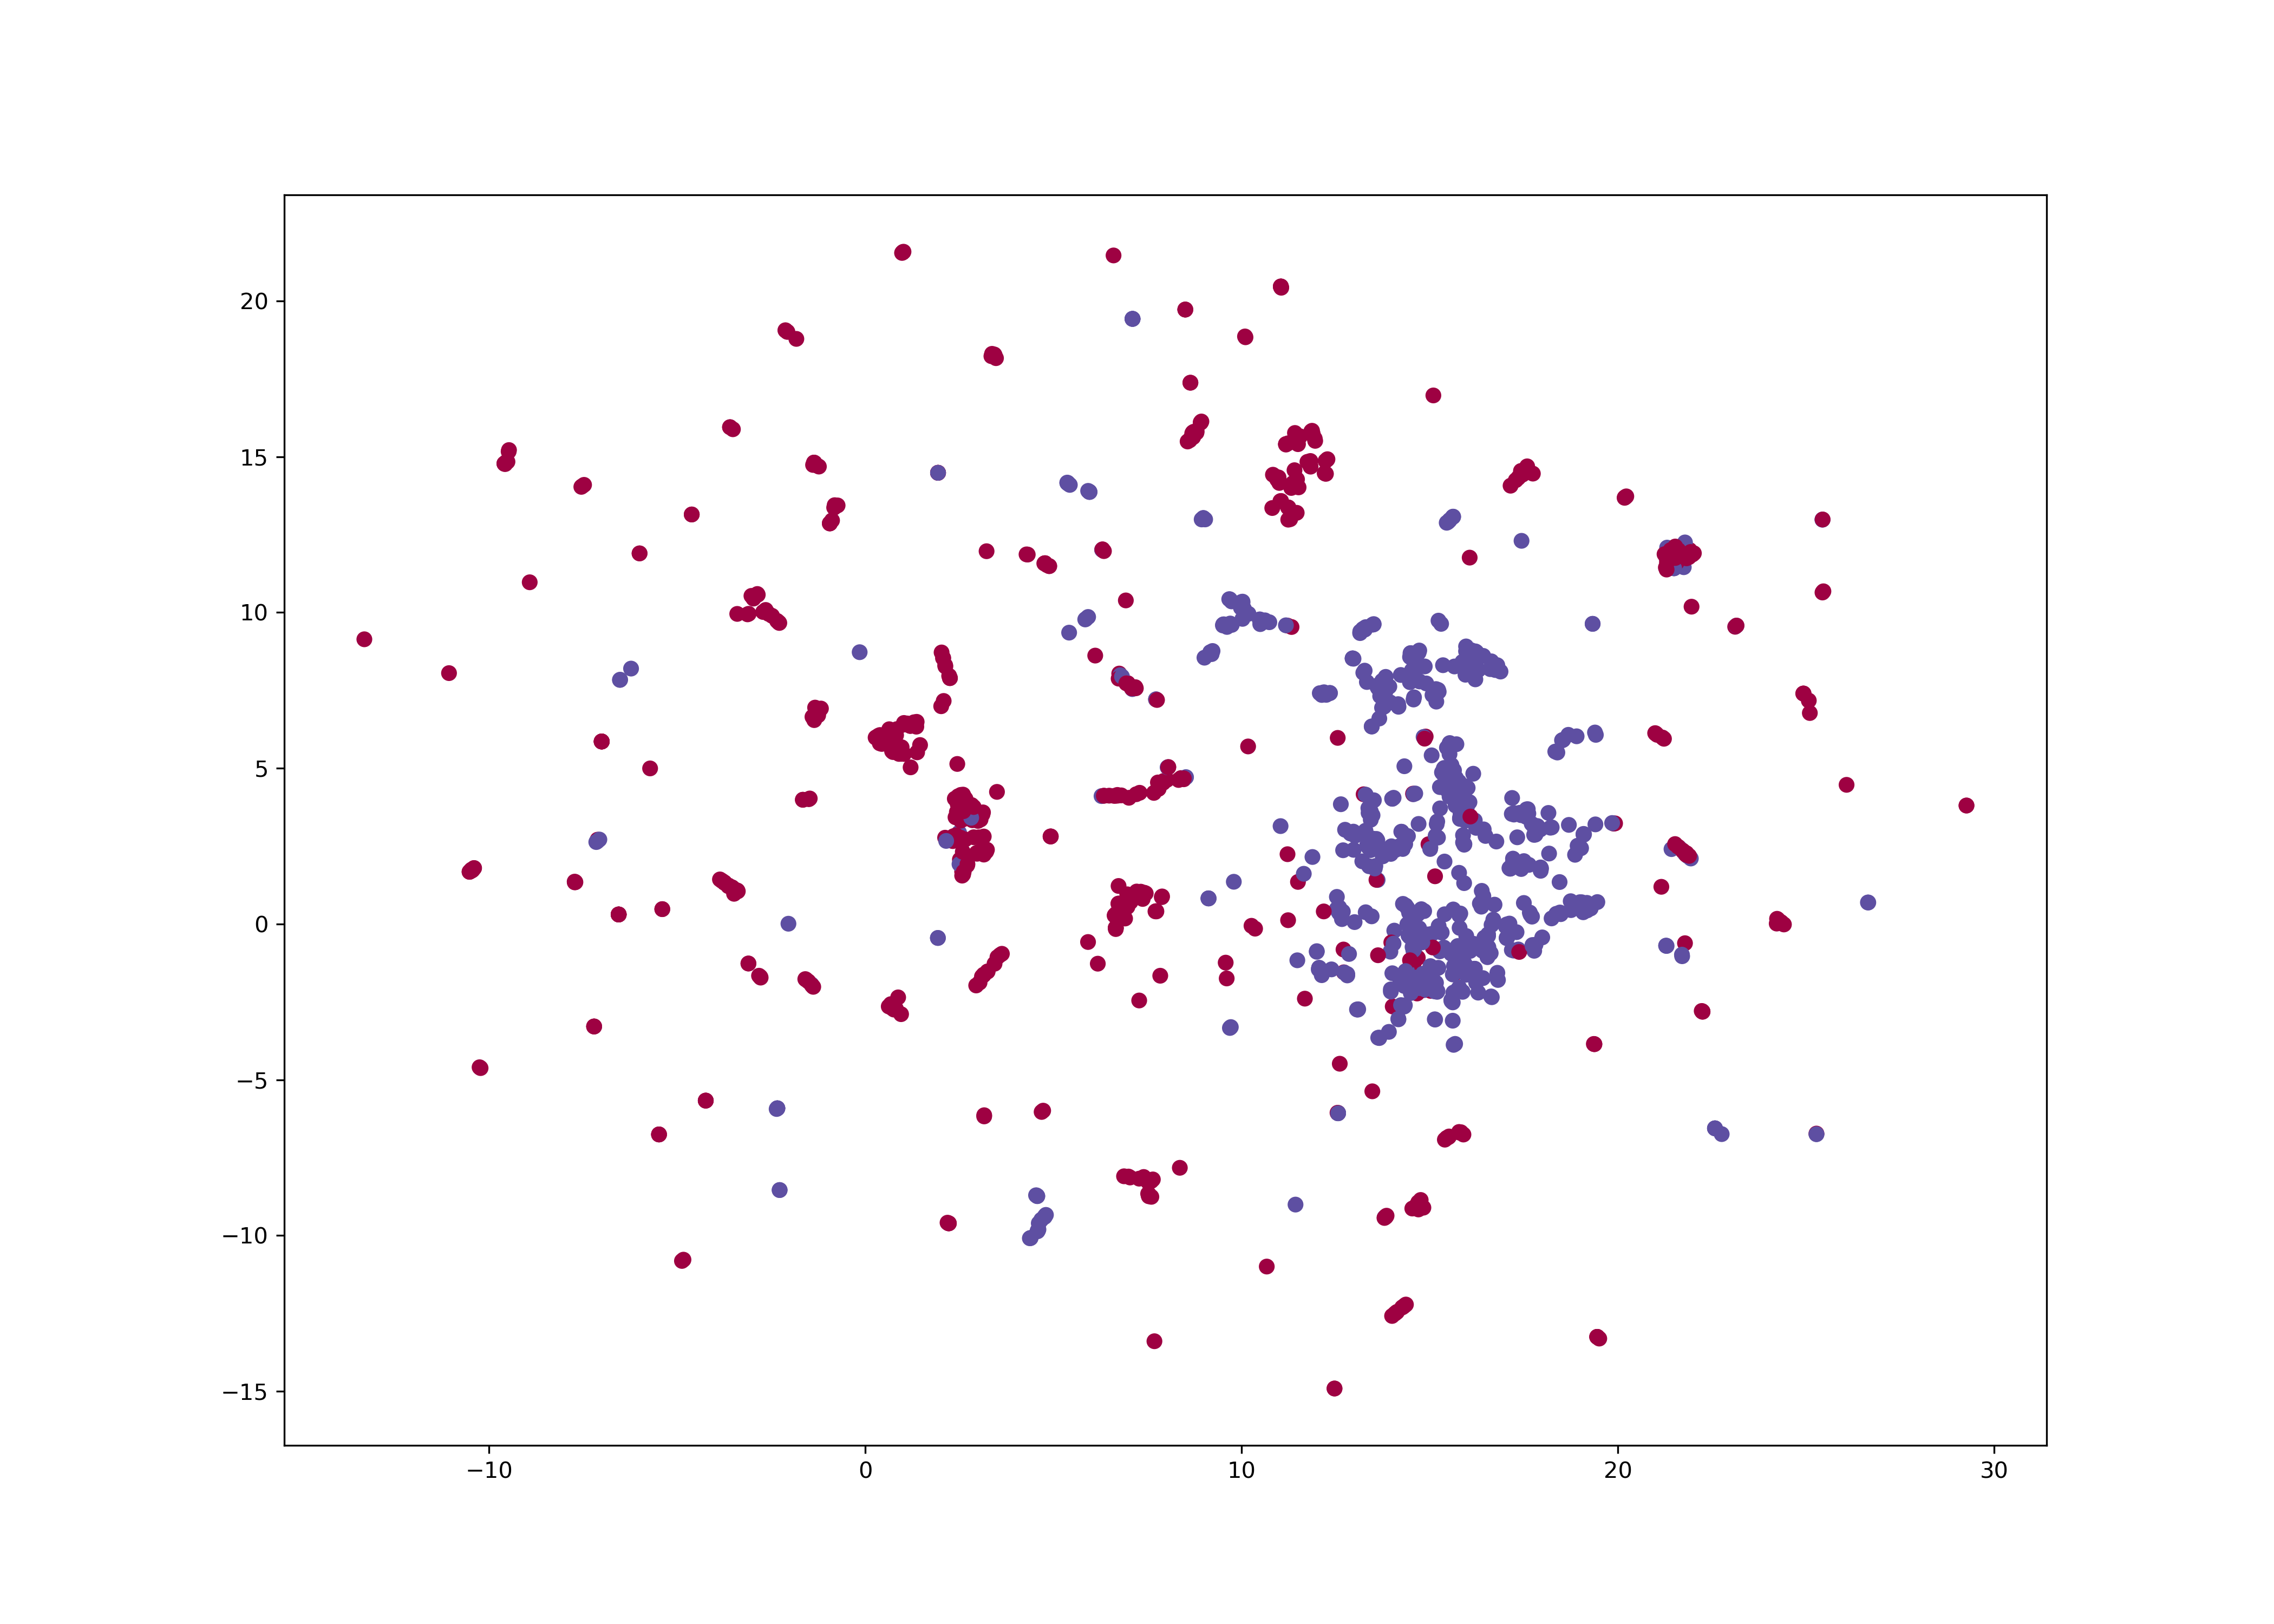
\includegraphics[width=0.5\textwidth,height=\textheight]{test_embedding.png}

}

\subcaption{\label{fig-umaptest}Projection of the Supervised UMAP on the
test set}

\end{minipage}%

\end{figure}%

Five neighbours and a Jaccard metric were then fed into a pipeline
together with a support vector machine classifier. A 10 fold stratified
cross validation approach was applied to assess performance. The mean
(standard deviation) of the CV test set balanced accuracy was found to
be 0.89 (0.017). The balanced accuracy of the test set that had been
held out was 0.888. The performance was reasonable given that structure
was expected to be a strong indicator of analogue suitability based the
Bayesian logistic regression findings and the fact that there was a
broad spread of Tanimoto indices across the similar and dissimilar
analogue pairs showing that complete separation based on structural
features alone was unlikely to be completely successful.

\subsection{Conclusions}\label{conclusions}

This compendium offers the potential to address a number of scientific
questions related to how past read-across assessments have been
performed and what future refinements are possible.


  \bibliography{references.bib}


\end{document}
